%%%%%%%%%%%%%%%%%%%%%%%%%%%%%%%%%%%%%%%%%%%%%%%%%%%%%%%%%%%%%%%%%%%%%%%%%%%%%%%%
%  Zawartość: Główny plik szablonu pracy dyplomowej (magisterskiej/inżynierskiej). 
%  Opracował: Tomasz Kubik <tomasz.kubik@pwr.edu.pl>
%  Data: styczeń 2023
%  Wersja: 0.9
%  Wymagania: kompilator pdflatex
%%%%%%%%%%%%%%%%%%%%%%%%%%%%%%%%%%%%%%%%%%%%%%%%%%%%%%%%%%%%%%%%%%%%%%%%%%%%%%%%

\documentclass[a4paper,onecolumn,oneside,12pt,extrafontsizes]{memoir}
%  W celu przygotowania wydruku do archiwum można:
%  a) przygotować pdf, w którym dwie strony zostaną wstawione na jedną fizyczną stronę i taki dokument wydrukować dwustronnie (podejście zalecane)
%
%   Taki dokument można przygotować poprzez
%   - wydruk z Adobe Acrobat Reader z opcją "Wiele" - sekcja "Rozmiar i obsługa stron"
%   - wykorzystanie narzędzi psutils
%
%      Windows (zakładając, że w dystrybucji MiKTeX jest pakiet miktex-psutils-bin-x64-2.9):
%        "c:\Program Files\MiKTeX 2.9\miktex\bin\x64\pdf2ps.exe" Dyplom.pdf Dyplom.ps
%        "c:\Program Files\MiKTeX 2.9\miktex\bin\x64\psnup.exe" -2 Dyplom.ps Dyplom2.ps
%        "c:\Program Files\MiKTeX 2.9\miktex\bin\x64\ps2pdf.exe" Dyplom2.ps Dyplom2.pdf
%        Del Dyplom2.ps Dyplom.ps
%
%     Linux:
%        pdf2ps Dyplom.pdf - | psnup -2 | ps2pdf - Dyplom2.pdf
%
%  b) przekomplilować dokument zmniejszając czcionkę (podejście niezalecane, bo zmienia formatowanie dokumentu)
%
%    Do tego wystarczy posłużyć się poniższymi komendami (zamiast documentclass z pierwszej linijki):
%   \documentclass[a4paper,onecolumn,twoside,10pt]{memoir} 
%   \renewcommand{\normalsize}{\fontsize{8pt}{10pt}\selectfont}

%\usepackage[cp1250]{inputenc} % Proszę zostawić, jeśli kodowanie edytowanych plików to cp1250 
\usepackage[utf8]{inputenc} % Proszę użyć zamiast powyższego, jeśli kodowanie edytowanych plików to UTF8
\usepackage[T1]{fontenc}
\usepackage[english,polish]{babel} % Tutaj ważna jest kolejność atrybutów (dla pracy po polsku polish powinno być na końcu)
%\DisemulatePackage{setspace}
\usepackage{setspace}
\usepackage{color,calc}
%\usepackage{soul} % pakiet z komendami do podkreślania, przekreślania, podświetlania tekstu (raczej niepotrzebny)
\usepackage{ebgaramond} % pakiet z czcionkami garamond, potrzebny tylko do strony tytułowej, musi wystąpić przed pakietem tgtermes

%% Aby uzyskać polskie literki w pdfie (a nie zlepki) korzystamy z pakietu czcionek tgterms. 
%% W pakiecie tym są zdefiniowane klony czcionek Times o kształtach: normalny, pogrubiony, italic, italic pogrubiony.
%% W pakiecie tym brakuje czcionki o kształcie: slanted (podobny do italic). 
%% Jeśli w dokumencie gdzieś zostanie zastosowana czcionka slanted (np. po użyciu komendy \textsl{}), to
%% latex dokona podstawienia na czcionkę standardową i zgłosi to w ostrzeżeniu (warningu).
%% Ponadto tgtermes to czcionka do tekstu. Wszelkie matematyczne wzory będą sformatowane domyślną czcionką do wzorów.
%% Jeśli wzory mają być sformatowane z wykorzystaniem innych czcionek, trzeba to jawnie zadeklarować.

%% Po zainstalowaniu pakietu tgtermes może będzie trzeba zauktualizować informacje 
%% o dostępnych fontach oraz mapy. Można to zrobić z konsoli (jako administrator)
%% initexmf --admin --update-fndb
%% initexmf --admin --mkmaps

\usepackage{tgtermes}   
\renewcommand*\ttdefault{txtt}


%%%%%%%%%%%%%%%%%%%%%%%%%%%%%%%%%%%%%%%%%%%%%%%%%%%%%%%%%%%%%%%%%%%%%%%%%%%%%%%%
%% Ustawienia odpowiedzialne za sposób łamania dokumentu
%% i ułożenie elementów pływających
%%%%%%%%%%%%%%%%%%%%%%%%%%%%%%%%%%%%%%%%%%%%%%%%%%%%%%%%%%%%%%%%%%%%%%%%%%%%%%%%
%\hyphenpenalty=10000		% nie dziel wyrazów zbyt często
\clubpenalty=10000      % kara za sierotki
\widowpenalty=10000     % nie pozostawiaj wdów
%\brokenpenalty=10000		% nie dziel wyrazów między stronami - trzeba było wyłączyć, bo nie łamały się linie w lstlisting
%\exhyphenpenalty=999999		% nie dziel słów z myślnikiem - trzeba było wyłączyć, bo nie łamały się linie w lstlisting
\righthyphenmin=3			  % dziel minimum 3 litery

%\tolerance=4500
%\pretolerance=250
%\hfuzz=1.5pt
%\hbadness=1450

\renewcommand{\topfraction}{0.95}
\renewcommand{\bottomfraction}{0.95}
\renewcommand{\textfraction}{0.05}
\renewcommand{\floatpagefraction}{0.35}

%%%%%%%%%%%%%%%%%%%%%%%%%%%%%%%%%%%%%%%%%%%%%%%%%%%%%%%%%%%%%%%%%%%%%%%%%%%%%%%%
%%  Ustawienia rozmiarów: tekstu, nagłówka i stopki, marginesów
%%  dla dokumentów klasy memoir 
%%%%%%%%%%%%%%%%%%%%%%%%%%%%%%%%%%%%%%%%%%%%%%%%%%%%%%%%%%%%%%%%%%%%%%%%%%%%%%%%
\setlength{\headsep}{10pt} 
\setlength{\headheight}{13.6pt} % wartość baselineskip dla czcionki 11pt tj. \small wynosi 13.6pt
\setlength{\footskip}{\headsep+\headheight}
\setlength{\uppermargin}{\headheight+\headsep+1cm}
\setlength{\textheight}{\paperheight-\uppermargin-\footskip-1.5cm}
\setlength{\textwidth}{\paperwidth-5cm}
\setlength{\spinemargin}{2.5cm}
\setlength{\foremargin}{2.5cm}
\setlength{\marginparsep}{2mm}
\setlength{\marginparwidth}{2.3mm}
%\settrimmedsize{297mm}{210mm}{*}
%\settrims{0mm}{0mm}	
\checkandfixthelayout[fixed] % konieczne, aby się dobrze wszystko poustawiało
%%%%%%%%%%%%%%%%%%%%%%%%%%%%%%%%%%%%%%%%%%%%%%%%%%%%%%%%%%%%%%%%%%%%%%%%%%%%%%%%
%%  Ustawienia odległości linii, wcięć, odstępów
%%%%%%%%%%%%%%%%%%%%%%%%%%%%%%%%%%%%%%%%%%%%%%%%%%%%%%%%%%%%%%%%%%%%%%%%%%%%%%%%
\linespread{1}
%\linespread{1.241}
\setlength{\parindent}{14.5pt}


\usepackage{multicol} % pakiet umożliwiający stworzenie wielokolumnowego tekstu
%%%%%%%%%%%%%%%%%%%%%%%%%%%%%%%%%%%%%%%%%%%%%%%%%%%%%%%%%%%%%%%%%%%%%%%%%%%%%%%%
%% Pakiety do formatowania tabel
%%%%%%%%%%%%%%%%%%%%%%%%%%%%%%%%%%%%%%%%%%%%%%%%%%%%%%%%%%%%%%%%%%%%%%%%%%%%%%%%
\usepackage{tabularx}
% Proszę używać tylko tabularx. Innych pakietów proszę nie stosować !!!
% Dokument na pewno da się zredagować bez ich użycia.
%\usepackage{longtable}
%\usepackage{ltxtable}
%\usepackage{tabulary}

%%%%%%%%%%%%%%%%%%%%%%%%%%%%%%%%%%%%%%%%%%%%%%%%%%%%%%%%%%%%%%%%%%%%%%%%%%%%%%%%
%% Pakiet do wstawiania fragmentów kodu
%%%%%%%%%%%%%%%%%%%%%%%%%%%%%%%%%%%%%%%%%%%%%%%%%%%%%%%%%%%%%%%%%%%%%%%%%%%%%%%%
\usepackage{listings} 
\usepackage{xpatch}
\makeatletter
\xpatchcmd\l@lstlisting{1.5em}{0em}{}{}
\makeatother
% Pakiet dostarcza otoczenia lstlisting. Jest ono wysoce konfigurowalne. 
% Konfigurować można indywidualnie każdy z listingów lub globalnie, w poleceniu \lstset{}.

% Zalecane jest, by kod źródłowy był wyprowadzany z użyciem czcionki maszynowej \ttfamily
% Ponieważ kod źródłowy, nawet po obcięciu do interesujących fragmentów, bywa obszerny, należy zmniejszyć czcionkę.
% Zalecane jest \small (dla krótkich fragmentów) oraz \footnotesize (dla dłuższych fragmentów).

% Ponadto podczas konfiguracji można zadeklarować sposób numerowania linii. Numerowanie linii zalecane jest jednak 
% tylko w przypadkach, gdy w redagowanym tekście znajdują się jakieś odwołania do konkretnych linii.
% Jeśli takich odwołań nie ma, numerowanie linii jest zbędne. Proszę wtedy go nie stosować.
% Przy włączaniu numerowania linii należy zwrócić uwagę na to, gdzie pojawią się te numery.
% Bez zmiany dodatkowych parametrów pojawiają się one na marginesie strony (co jest niepożądane).

\lstset{
  basicstyle=\small\ttfamily, % lub basicstyle=\footnotesize\ttfamily
  %%columns=fullflexible,
	%%showstringspaces=false,
	%%showspaces=false,
  breaklines=true,
  postbreak=\mbox{\textcolor{red}{$\hookrightarrow$}\space}, 
  %%numbers=left,  % ta i poniższe linie dotyczą ustawienia numerowania i sposobu jego wyprowadzania
  %%firstnumber=1, 
  %%numberfirstline=true, 
	%%xleftmargin=17pt,
  %%framexleftmargin=17pt,
  %%framexrightmargin=5pt,
  %%framexbottommargin=4pt,
	belowskip=.5\baselineskip,
	literate={\_}{{\_\allowbreak}}1 % ta deklaracja przydaje się, jeśli na listingu mają być łamane nazwy zawierające podkreślniki
}

% Jeśli edytowany plik nie jest w kodowaniu cp1250, to jest problem z polskimi znakami występującymi we wstawianym kodzie.
% Dlatego podczas pracy na plikach w kodowaniu UTF8 trzeba zadeklarować mapowanie jak niżej (wystarczy odmarkować).
% Niestety, jak się zastosuje to mapowanie mogą pojawić się problemy z podświetlaniem składni (patrz dalej).
\lstset{literate=%-
{ą}{{\k{a}}}1 {ć}{{\'c}}1 {ę}{{\k{e}}}1 {ł}{{\l{}}}1 {ń}{{\'n}}1 {ó}{{\'o}}1 {ś}{{\'s}}1 {ż}{{\.z}}1 {ź}{{\'z}}1 {Ą}{{\k{A}}}1 {Ć}{{\'C}}1 {Ę}{{\k{E}}}1 {Ł}{{\L{}}}1 {Ń}{{\'N}}1 {Ó}{{\'O}}1 {Ś}{{\'S}}1 {Ż}{{\.Z}}1 {Ź}{{\'Z}}1 
    {Ö}{{\"O}}1
    {Ä}{{\"A}}1
    {Ü}{{\"U}}1
    {ß}{{\ss}}1
    {ü}{{\"u}}1
    {ä}{{\"a}}1
    {ö}{{\"o}}1
    {~}{{\textasciitilde}}1
		{—}{{{\textemdash} }}1
}%{\ \ }{{\ }}1}


%% lstlisting pozwala na ostylowania podświetlania składni wybranych języków.
%% Działa to na zasadzie zdefiniowania słów kluczowych oraz sposobu ich wyświetlania.
%% Ponieważ jest to prosty mechanizm, czasem trudno osiągnąć takie efekty, jakie dają narzędzia IDE. 
%% Jednak w większości przypadku osiągane rezutlaty są zadowalające.


%% lstlisting obsługuje domyślnie kilka najpopularniejszych języków.
%%\lstloadlanguages{% Check Dokumentation for further languages ...
%%C,
%%C++,
%%csh,
%%Java
%%}
%% Inne języki muszą być dodefiniowane. Poniżej podano przykłady definicji języków i styli.

\definecolor{lightgray}{rgb}{.9,.9,.9}
\definecolor{darkgray}{rgb}{.4,.4,.4}
\definecolor{purple}{rgb}{0.65, 0.12, 0.82}
\definecolor{javared}{rgb}{0.6,0,0} % for strings
\definecolor{javagreen}{rgb}{0.25,0.5,0.35} % comments
\definecolor{javapurple}{rgb}{0.5,0,0.35} % keywords
\definecolor{javadocblue}{rgb}{0.25,0.35,0.75} % javadoc
 
\lstdefinelanguage{JavaScript}{ 
	keywords={typeof, new, true, false, catch, function, return, null, catch, switch, var, if, in, while, do, else, case, break},
	keywordstyle=\color{blue}\bfseries,
	ndkeywords={class, export, boolean, throw, implements, import, this},
	ndkeywordstyle=\color{darkgray}\bfseries,
	identifierstyle=\color{black},
	sensitive=false,
	comment=[l]{//},
	morecomment=[s]{/*}{*/},
	commentstyle=\color{purple}\ttfamily,
	stringstyle=\color{red}\ttfamily,
	morestring=[b]',
	morestring=[b]"
}
\lstdefinestyle{JavaScriptStyle}{
	language=JavaScript,
	commentstyle=\color{javagreen}, % niestety, jeśli w linii komentarza pojawią się słowa kluczowe, to zostaną pokolorowane
	backgroundcolor=,%\color{lightgray}, % można ustwić kolor tła, ale jest to niezalecane
	extendedchars=true,
	basicstyle=\footnotesize\ttfamily,
	showstringspaces=false,
	showspaces=false,
	numbers=none,%left,
	numberstyle=\footnotesize,
	numbersep=9pt,
	tabsize=2,
	breaklines=true,
	showtabs=false,
	captionpos=t
}

\lstdefinestyle{JavaStyle}{
basicstyle=\footnotesize\ttfamily,
keywordstyle=\color{javapurple}\bfseries,
stringstyle=\color{javared},
commentstyle=\color{javagreen},
morecomment=[s][\color{javadocblue}]{/**}{*/},
numbers=none,%left,
numberstyle=\tiny\color{black},
stepnumber=2,
numbersep=10pt,
tabsize=4,
showspaces=false,
showstringspaces=false,
captionpos=t
}

\definecolor{pblue}{rgb}{0.13,0.13,1}
\definecolor{pgreen}{rgb}{0,0.5,0}
\definecolor{pred}{rgb}{0.9,0,0}
\definecolor{pgrey}{rgb}{0.46,0.45,0.48}
\definecolor{dark-grey}{rgb}{0.4,0.4,0.4}
% styl json
\newcommand\JSONnumbervaluestyle{\color{blue}}
\newcommand\JSONstringvaluestyle{\color{red}}

\newif\ifcolonfoundonthisline

\makeatletter

\lstdefinestyle{json-style}  
{
	showstringspaces    = false,
	keywords            = {false,true},
	alsoletter          = 0123456789.,
	morestring          = [s]{"}{"},
	stringstyle         = \ifcolonfoundonthisline\JSONstringvaluestyle\fi,
	MoreSelectCharTable =%
	\lst@DefSaveDef{`:}\colon@json{\processColon@json},
	basicstyle          = \footnotesize\ttfamily,
	keywordstyle        = \ttfamily\bfseries,
	numbers				= left, % zakomentować, jeśli numeracja linii jest niepotrzebna
	numberstyle={\footnotesize\ttfamily\color{dark-grey}},
	xleftmargin			= 2em % zakomentować, jeśli numeracja linii jest niepotrzebna
}

\newcommand\processColon@json{%
	\colon@json%
	\ifnum\lst@mode=\lst@Pmode%
	\global\colonfoundonthislinetrue%
	\fi
}

\lst@AddToHook{Output}{%
	\ifcolonfoundonthisline%
	\ifnum\lst@mode=\lst@Pmode%
	\def\lst@thestyle{\JSONnumbervaluestyle}%
	\fi
	\fi
	\lsthk@DetectKeywords% 
}

\lst@AddToHook{EOL}%
{\global\colonfoundonthislinefalse}

\makeatother

%%\definecolor{red}{rgb}{0.6,0,0} % for strings
%%\definecolor{blue}{rgb}{0,0,0.6}
%%\definecolor{green}{rgb}{0,0.8,0}
%%\definecolor{cyan}{rgb}{0.0,0.6,0.6}
%%
%%\lstdefinestyle{sqlstyle}{
%%language=SQL,
%%basicstyle=\footnotesize\ttfamily, 
%%numbers=left, 
%%numberstyle=\tiny, 
%%numbersep=5pt, 
%%tabsize=2, 
%%extendedchars=true, 
%%breaklines=true, 
%%showspaces=false, 
%%showtabs=true, 
%%xleftmargin=17pt,
%%framexleftmargin=17pt,
%%framexrightmargin=5pt,
%%framexbottommargin=4pt,
%%keywordstyle=\color{blue}, 
%%commentstyle=\color{green}, 
%%stringstyle=\color{red}, 
%%}
%%
%%\lstdefinestyle{sharpcstyle}{
%%language=[Sharp]C,
%%basicstyle=\footnotesize\ttfamily, 
%%numbers=left, 
%%numberstyle=\tiny, 
%%numbersep=5pt, 
%%tabsize=2, 
%%extendedchars=true, 
%%breaklines=true, 
%%showspaces=false, 
%%showtabs=true, 
%%xleftmargin=17pt,
%%framexleftmargin=17pt,
%%framexrightmargin=5pt,
%%framexbottommargin=4pt,
%%morecomment=[l]{//}, %use comment-line-style!
%%morecomment=[s]{/*}{*/}, %for multiline comments
%%showstringspaces=false, 
%%morekeywords={  abstract, event, new, struct,
                %%as, explicit, null, switch,
                %%base, extern, object, this,
                %%bool, false, operator, throw,
                %%break, finally, out, true,
                %%byte, fixed, override, try,
                %%case, float, params, typeof,
                %%catch, for, private, uint,
                %%char, foreach, protected, ulong,
                %%checked, goto, public, unchecked,
                %%class, if, readonly, unsafe,
                %%const, implicit, ref, ushort,
                %%continue, in, return, using,
                %%decimal, int, sbyte, virtual,
                %%default, interface, sealed, volatile,
                %%delegate, internal, short, void,
                %%do, is, sizeof, while,
                %%double, lock, stackalloc,
                %%else, long, static,
                %%enum, namespace, string},
%%keywordstyle=\color{cyan},
%%identifierstyle=\color{red},
%%stringstyle=\color{blue}, 
%%commentstyle=\color{green},
%%}



%%%%%%%%%%%%%%%%%%%%%%%%%%%%%%%%%%%%%%%%%%%%%%%%%%%%%%%%%%%%%%%%%%%%%%%%%%%%%%%%
%%  Pakiety i komendy zastosowane tylko do zamieszczenia informacji o użytych komendach i fontach w tym szablonie.
%%  Normalnie nie są one potrzebne. Proszę poniższe deklaracje zamarkować podczas redakcji pracy !!!!
%%%%%%%%%%%%%%%%%%%%%%%%%%%%%%%%%%%%%%%%%%%%%%%%%%%%%%%%%%%%%%%%%%%%%%%%%%%%%%%%
%%\usepackage{memlays}     % extra layout diagrams, zastosowane w szblonie do 'debuggowania', używa pakietu layouts
%%%\usepackage{layouts}
%%\usepackage{printlen} % pakiet do wyświetlania wartości zdefiniowanych długości, stosowany do 'debuggowania'
%%\usepackage{enumitem} % pakiet do numerowania 1.1 1.2 w sekcji enumrate
%%\uselengthunit{pt}
%%\makeatletter
%%\newcommand{\showFontSize}{\f@size pt} % makro wypisujące wielkość bieżącej czcionki
%%\makeatother
% do pokazania ramek można byłoby użyć:
%\usepackage{showframe} 

%%%%%%%%%%%%%%%%%%%%%%%%%%%%%%%%%%%%%%%%%%%%%%%%%%%%%%%%%%%%%%%%%%%%%%%%%%%%%%%%
%%  Formatowanie list wyliczeniowych, wypunktowań i własnych otoczeń
%%%%%%%%%%%%%%%%%%%%%%%%%%%%%%%%%%%%%%%%%%%%%%%%%%%%%%%%%%%%%%%%%%%%%%%%%%%%%%%%

% Domyślnie wypunktowania mają zadeklarowane znaki, które nie występują w tgtermes
% Aby latex nie podstawiał w ich miejsca znaków z czcionki standardowej można zrobić podstawienie:
%    \DeclareTextCommandDefault{\textbullet}{\ensuremath{\bullet}}
%    \DeclareTextCommandDefault{\textasteriskcentered}{\ensuremath{\ast}}
%    \DeclareTextCommandDefault{\textperiodcentered}{\ensuremath{\cdot}}
% Jednak jeszcze lepszym pomysłem jest zdefiniowanie otoczeń z wykorzystaniem enumitem
\usepackage{enumitem} % pakiet pozwalający zarządzać formatowaniem list wyliczeniowych
\setlist{noitemsep,topsep=4pt,parsep=0pt,partopsep=4pt,leftmargin=*} % zadeklarowane parametry pozwalają uzyskać 'zwartą' postać wypunktowania bądź wyliczenia
\setenumerate{labelindent=0pt,itemindent=0pt,leftmargin=!,label=\arabic*.} % można zmienić \arabic na \alph, jeśli wyliczenia mają być z literkami
\setlistdepth{4} % definiujemy głębokość zagnieżdżenia list wyliczeniowych do 4 poziomów
\setlist[itemize,1]{label=$\bullet$}  % definiujemy, jaki symbol ma być użyty w wyliczeniu na danym poziomie
\setlist[itemize,2]{label=\normalfont\bfseries\textendash}
\setlist[itemize,3]{label=$\ast$}
\setlist[itemize,4]{label=$\cdot$}
\renewlist{itemize}{itemize}{4}

%%%http://tex.stackexchange.com/questions/29322/how-to-make-enumerate-items-align-at-left-margin
%\renewenvironment{enumerate}
%{
%\begin{list}{\arabic{enumi}.}
%{
%\usecounter{enumi}
%%\setlength{\itemindent}{0pt}
%%\setlength{\leftmargin}{1.8em}%{2zw} % 
%%\setlength{\rightmargin}{0zw} %
%%\setlength{\labelsep}{1zw} %
%%\setlength{\labelwidth}{3zw} % 
%\setlength{\topsep}{6pt}%
%\setlength{\partopsep}{0pt}%
%\setlength{\parskip}{0pt}%
%\setlength{\parsep}{0em} % 
%\setlength{\itemsep}{0em} % 
%%\setlength{\listparindent}{1zw} % 
%}
%}{
%\end{list}
%}

\makeatletter
\renewenvironment{quote}{
	\begin{list}{}
	{
	\setlength{\leftmargin}{1em}
	\setlength{\topsep}{0pt}%
	\setlength{\partopsep}{0pt}%
	\setlength{\parskip}{0pt}%
	\setlength{\parsep}{0pt}%
	\setlength{\itemsep}{0pt}
	}
	}{
	\end{list}}
\makeatother

%%%%%%%%%%%%%%%%%%%%%%%%%%%%%%%%%%%%%%%%%%%%%%%%%%%%%%%%%%%%%%%%%%%%%%%%%%%%%%%%
%%  Pakiet i komendy do generowania indeksu 
%% (ważne, by pojawiły się przed pakietem hyperref)
%%%%%%%%%%%%%%%%%%%%%%%%%%%%%%%%%%%%%%%%%%%%%%%%%%%%%%%%%%%%%%%%%%%%%%%%%%%%%%%%
% pdftex jest w stanie wygenerować indeks (czyli spis haseł z referencjami do stron, na których te hasła się pojawiły).
% Generalnie z indeksem jest sporo problemów, zwłaszcza, gdy pojawiają się polskie literki.
% Trzeba wtedy korzystać z xindy.
% Zwykle w pracach dyplomowych indeksy nie są wykorzystywane. Dlatego są zamarkowane.
%\DisemulatePackage{imakeidx}
%\usepackage[makeindex,noautomatic]{imakeidx} % tutaj mówimy, żeby indeks nie generował się automatycznie, 
%\makeindex
%
%\makeatletter
%%%%\renewenvironment{theindex}
							 %%%%{\vskip 10pt\@makeschapterhead{\indexname}\vskip -3pt%
								%%%%\@mkboth{\MakeUppercase\indexname}%
												%%%%{\MakeUppercase\indexname}%
								%%%%\vspace{-3.2mm}\parindent\z@%
								%%%%\renewcommand\subitem{\par\hangindent 16\p@ \hspace*{0\p@}}%%
								%%%%\phantomsection%
								%%%%\begin{multicols}{2}
								%%%%%\thispagestyle{plain}
								%%%%\parindent\z@                
								%%%%%\parskip\z@ \@plus .3\p@\relax
								%%%%\let\item\@idxitem}
							 %%%%{\end{multicols}\clearpage}
%%%%
%\makeatother




%%%%%%%%%%%%%%%%%%%%%%%%%%%%%%%%%%%%%%%%%%%%%%%%%%%%%%%%%%%%%%%%%%%%%%%%%%%%%%%%
%%  Sprawy metadanych w wynikowym pdf, hyperlinków itp.
%%%%%%%%%%%%%%%%%%%%%%%%%%%%%%%%%%%%%%%%%%%%%%%%%%%%%%%%%%%%%%%%%%%%%%%%%%%%%%%%
% Szablon przygotowano głównie dla pdflatex. Specyficzne komendy dla pdf-owej kompilacj wstawiono 
% w instrukcję warunkową dostarczaną przez pakiet ifpdf 
% Jeśli metadane zawierają przecinki lub średniki, domyślnie metadane te otaczane są apostrofami.
% Piszą o tym na stronie: https://tex.stackexchange.com/questions/3708/hyperref-enquotes-metadata
% Aby pozbyć się tych apostrofów użyto pakietu hyperxmp (ładującego kilka innych pakietów)
\usepackage{hyperxmp}
\usepackage{ifpdf}
%\newif\ifpdf \ifx\pdfoutput\undefined
%\pdffalse % we are not running PDFLaTeX
%\else
%\pdfoutput=1 % we are running PDFLaTeX
%\pdftrue \fi
\ifpdf
 \usepackage{datetime2} % INFO: pakiet potrzeby do uzyskania i sformatowania daty 
 \usepackage[pdftex,bookmarks,breaklinks,unicode]{hyperref}
 \usepackage[pdftex]{graphicx}
 \DeclareGraphicsExtensions{.pdf,.jpg,.mps,.png} % po zadeklarowaniu rozszerzeń można będzie wstawiać pliki z grafiką bez konieczności podawania tych rozszerzeń w ich nazwach
\pdfcompresslevel=9
\pdfoutput=1

% Dobrze przygotowany dokument pdf to taki, który zawiera metadane.
% Poniżej zadeklarowano pola metadanych, jakie będą włączone do dokumentu pdf.
% Można je zmodyfikować w zależności od potrzeb
\makeatletter
\AtBeginDocument{  
  \hypersetup{
	pdfinfo={
    Title = {\@title},
    Author = {\@author},
    Subject={Praca dyplomowa \ifMaster magisterska\else inżynierska\fi},  
    Keywords={\@kvpl}, 
		Producer={}, 
	  CreationDate= {}, % należy wstawiać zgodnie ze składnią: {D:yyyymmddhhmmss}, np. D:20210208175600
    ModDate={\pdfcreationdate},   % data modyfikacji będzie datą kompilacji
		Creator={pdftex},
	}}
}
\pdftrailerid{} %Remove ID
\pdfsuppressptexinfo15 %Suppress PTEX.Fullbanner and info of imported PDFs
\makeatother
\else             % jeśli kompilacja jest inna niż pdflatex
\usepackage{graphicx}
\DeclareGraphicsExtensions{.eps,.ps,.jpg,.mps,.png}
\fi
\sloppy

% INFO: dodane by lepiej łamać urle 
\def\UrlBreaks{\do\/\do-\do_} 
% INFO: choć można zadeklarować foldery, w jakich pojawiać się mają pliki z grafiką, zaleca się jednak, by tego nie robić
%\graphicspath{{rys01/}{rys02/}}  


%%%%%%%%%%%%%%%%%%%%%%%%%%%%%%%%%%%%%%%%%%%%%%%%%%%%%%%%%%%%%%%%%%%%%%%%%%%%%%%%
%%  Formatowanie dokumentu
%%%%%%%%%%%%%%%%%%%%%%%%%%%%%%%%%%%%%%%%%%%%%%%%%%%%%%%%%%%%%%%%%%%%%%%%%%%%%%%%
% INFO: Deklaracja głębokościu numeracji
\setcounter{secnumdepth}{2}
\setcounter{tocdepth}{2}
\setsecnumdepth{subsection} 
% INFO: Dodanie kropek po numerach sekcji
\makeatletter
\def\@seccntformat#1{\csname the#1\endcsname.\quad}
\def\numberline#1{\hb@xt@\@tempdima{#1\if&#1&\else.\fi\hfil}}
\makeatother
% INFO: Numeracja rozdziałów i separatory
\renewcommand{\chapternumberline}[1]{#1.\quad}
\renewcommand{\cftchapterdotsep}{\cftdotsep}


%\usepackage{etoolbox} % odstępy w spisie treści (jeden ze sposobów ustawiania)
%%\makeatletter
%%\pretocmd{\chapter}{\addtocontents{toc}{\protect\addvspace{-1\p@}}}{}{}
%%\pretocmd{\section}{\addtocontents{toc}{\protect\addvspace{-1\p@}}}{}{}
%%\pretocmd{\subsection}{\addtocontents{toc}{\protect\addvspace{-1\p@}}}{}{}
%%\makeatother

\makeatletter % odstępy w spisie pomiędzy rozdziałami
\renewcommand*{\insertchapterspace}{%
  \addtocontents{lof}{\protect\addvspace{3pt}}%
  \addtocontents{lot}{\protect\addvspace{3pt}}%
	\addtocontents{toc}{\protect\addvspace{3pt}} %
  \addtocontents{lol}{\protect\addvspace{3pt}}}
\makeatother 


\setlength{\cftbeforechapterskip}{0pt} % odstępy w spisie treści przed rozdziałem, działa w korelacji z:
\renewcommand{\aftertoctitle}{\afterchaptertitle\vspace{-4pt}} % 
% https://stackoverflow.com/questions/3029271/latex-make-listoffigures-look-like-listoftables-or-lstlistoflistings
%\renewcommand{\memchapinfo}[4]{%
%  \addtocontents{lol}{\protect\addvspace{10pt}}
%}

%\cftsetindents{section}{1.5em}{2.3em}

%\setbeforesecskip{10pt plus 0.5ex}%{-3.5ex \@plus -1ex \@minus -.2ex}
%\setaftersecskip{10pt plus 0.5ex}%\onelineskip}
%\setbeforesubsecskip{8pt plus 0.5ex}%{-3.5ex \@plus -1ex \@minus -.2ex}
%\setaftersubsecskip{8pt plus 0.5ex}%\onelineskip}
%\setlength\floatsep{6pt plus 2pt minus 2pt} 
%\setlength\intextsep{12pt plus 2pt minus 2pt} 
%\setlength\textfloatsep{12pt plus 2pt minus 2pt} 

% Ustawienie odstępu od góry w nienumerowanych rozdziałach oraz wykazach:
% Spis treści, Spis tabel, Spis rysunków, Indeks rzeczowy
%\newlength{\linespace}
%\setlength{\linespace}{-\beforechapskip-\topskip+\headheight+\topsep}
%%%\makechapterstyle{noNumbered}{%
%%%\renewcommand\chapterheadstart{\vspace*{\linespace}}
%%%}
%% powyższa komenda załatwia to, co robią komendy poniższe dla spisów
%\renewcommand*{\tocheadstart}{\vspace*{\linespace}}
%\renewcommand*{\lotheadstart}{\vspace*{\linespace}}
%\renewcommand*{\lofheadstart}{\vspace*{\linespace}}


% INFO: Czcionka do podpisów tabel, rysunków, listingów
\captionnamefont{\small}
\captiontitlefont{\small}


% INFO: Sformatowanie podpisu nad dwukolumnowym listingiem
\newcommand{\listingcaption}[1]
{%
\vspace*{\abovecaptionskip}\small 
\refstepcounter{lstlisting}\hfill%
Listing \thelstlisting: #1\hfill%\hfill%
\addcontentsline{lol}{lstlisting}{\protect\numberline{\thelstlisting}#1}
}%



% INFO: Pomocnicze marko do wyróżniania tekstu w języku angielskim
\newcommand{\eng}[1]{(ang.~\emph{#1})}
% IFNO: Pomocnicze makro do dołączania podpisów do rysunków ze wskazaniem źródła (bez wypisywania tego źródła w spisie rysunków)
\newcommand*{\captionsource}[2]{%
  \caption[{#1}]{%
    #1 \emph{Źródło:} #2%
  }%
}


% INFO: Makro pozwalające zmienić sposób wypisywania rozdziału (proszę z niego nie korzystać)
%\def\printchaptertitle##1{\fonttitle \space \thechapter.\space ##1} 

% INFO: definicje etykiet i tytułów spisów

%\AtBeginDocument{% 
        \addto\captionspolish{% 
        \renewcommand{\tablename}{Tab.}%% INFO: Przedefiniowanie etykiet w podpisach tabel 
}%} 

%\AtBeginDocument{% 
%        \addto\captionspolish{% 
%        \renewcommand{\chaptername}{Rozdział}% INFO: Przedefiniowanie nazwy rozdziału, niepotrzebne, bo przy polskich ustawieniach językowych jest 'Rozdział'
%}} 

% Przedefiniowanie etykiet oraz nazw wykazu literatury, spisów, indeksu
%\AtBeginDocument{% 
        \addto\captionspolish{% 
        \renewcommand{\figurename}{Rys.}%% INFO: Przedefiniowanie etykiet w podpisach rysunków 
}%}

%\AtBeginDocument{% 
        \addto\captionspolish{% 
        \renewcommand{\lstlistlistingname}{Spis listingów}%% INFO: Przedefiniowanie nazwy spisu listingów
}%} 
\newlistof{lstlistoflistings}{lol}{\lstlistlistingname}


%\AtBeginDocument{% 
        \addto\captionspolish{% 
        \renewcommand{\bibname}{Literatura}%% INFO: Przedefiniowanie nazwy wykazu literatury 
}%}

%\AtBeginDocument{% 
        \addto\captionspolish{% 
        \renewcommand{\listfigurename}{Spis rysunków}%% INFO: Przedefiniowanie nazwy spisu rysunków 
}%}

%\AtBeginDocument{% 
        \addto\captionspolish{% 
        \renewcommand{\listtablename}{Spis tabel}%% INFO: Przedefiniowanie nazwy spisu tabel 
}%}

%\AtBeginDocument{% 
        \addto\captionspolish{% 
\renewcommand\indexname{Indeks rzeczowy}%% INFO: Przedefiniowanie nazwy indeksu 
}%}

%\AtBeginDocument{% 
%    \addto\captionspolish{
%\renewcommand\abstractname{Streszczenie}%% INFO: Przedefiniowanie nazwy strzeszczenia, niepotrzebne, bo przy polskich ustawieniach językowych jest 'Streszczenie'
%}%}

%\AtBeginDocument{% 
%    \addto\captionsenglish{
%\renewcommand\abstractname{Abstract} 
%}%}

\renewcommand{\abstractnamefont}{\normalfont\Large\bfseries}
\renewcommand{\abstracttextfont}{\normalfont}


%%%%%%%%%%%%%%%%%%%%%%%%%%%%%%%%%%%%%%%%%%%%%%%%%%%%%%%%%%%%%%%%%%%%%%%%%%%%%%%%
%% Definicje stopek i nagłówków
%%%%%%%%%%%%%%%%%%%%%%%%%%%%%%%%%%%%%%%%%%%%%%%%%%%%%%%%%%%%%%%%%%%%%%%%%%%%%%%%
\addtopsmarks{headings}{%
\nouppercaseheads % added at the beginning
}{%
\createmark{chapter}{both}{shownumber}{}{. \space}
%\createmark{chapter}{left}{shownumber}{}{. \space}
\createmark{section}{right}{shownumber}{}{. \space}
}%use the new settings

\makeatletter
\copypagestyle{outer}{headings}
\makeoddhead{outer}{}{}{\small\itshape\rightmark}
\makeevenhead{outer}{\small\itshape\leftmark}{}{}
\makeoddfoot{outer}{\small\@author:~\@titleShort}{}{\small\thepage}
\makeevenfoot{outer}{\small\thepage}{}{\small\@author:~\@title}
\makeheadrule{outer}{\linewidth}{\normalrulethickness}
\makefootrule{outer}{\linewidth}{\normalrulethickness}{2pt}
\makeatother

% fix plain
\copypagestyle{plain}{headings} % overwrite plain with outer
\makeoddhead{plain}{}{}{} % remove right header
\makeevenhead{plain}{}{}{} % remove left header
\makeevenfoot{plain}{}{}{}
\makeoddfoot{plain}{}{}{}

\copypagestyle{empty}{headings} % overwrite plain with outer
\makeoddhead{empty}{}{}{} % remove right header
\makeevenhead{empty}{}{}{} % remove left header
\makeevenfoot{empty}{}{}{}
\makeoddfoot{empty}{}{}{}

% INFO: deklaracja zmiennej logicznej wykorzystywanej do rozróżnienia pracy inżynierskiej i magisterskiej
\newif\ifMaster% domyślnie false (czyli domyślnie mamy pracę inżynierską)

%%%%%%%%%%%%%%%%%%%%%%%%%%%%%%%%%%%%%%%%%%%%%%%%%%%%%%%%%%%%%%%%%%%%%%%%%%%%%%%%
%% Definicja strony tytułowej 
%%%%%%%%%%%%%%%%%%%%%%%%%%%%%%%%%%%%%%%%%%%%%%%%%%%%%%%%%%%%%%%%%%%%%%%%%%%%%%%%
\makeatletter
%Uczelnia
\newcommand\uczelnia[1]{\renewcommand\@uczelnia{#1}}
\newcommand\@uczelnia{}
%Wydział
\newcommand\wydzial[1]{\renewcommand\@wydzial{#1}}
\newcommand\@wydzial{}
%Kierunek
\newcommand\kierunek[1]{\renewcommand\@kierunek{#1}}
\newcommand\@kierunek{}
%Specjalność
\newcommand\specjalnosc[1]{\renewcommand\@specjalnosc{#1}}
\newcommand\@specjalnosc{}
%Tytuł po angielsku
\newcommand\titleEN[1]{\renewcommand\@titleEN{#1}}
\newcommand\@titleEN{}
%Tytuł krótki
\newcommand\titleShort[1]{\renewcommand\@titleShort{#1}}
\newcommand\@titleShort{}
%Promotor
\newcommand\promotor[1]{\renewcommand\@promotor{#1}}
\newcommand\@promotor{}
%Słowa kluczowe
\newcommand\kvpl[1]{\renewcommand\@kvpl{#1}}
\newcommand\@kvpl{}
\newcommand\kven[1]{\renewcommand\@kven{#1}}
\newcommand\@kven{}
%Komenda wykorzystywana w streszczeniu
\newcommand\mykeywords{\hspace{\absleftindent}%
\parbox{\linewidth-2.0\absleftindent}{
       \iflanguage{polish}{\textbf{Słowa kluczowe:} \@kvpl}{%
			 \iflanguage{english}{\textbf{Keywords:} \@kven}}{}}
				}

\def\maketitle{%
  \pagestyle{empty}%
%%\garamond 
	\fontfamily{\ebgaramond@family}\selectfont % na stronie tytułowej czcionka garamond
%%%%%%%%%%%%%%%%%%%%%%%%%%%%%%%%%%%%%%%%%%%%%%%%%%%%%%%%%%%%%%%%%%%%%%%%%%%%%%	
%% Poniżej, w otoczniu picture, wstawiono tytuł i autora. 
%% Tytuł (z autorem) musi znaleźć się w obszarze 
%% odpowiadającym okienku 110mmx75mm, którego lewy górny róg 
%% jest w położeniu 77mm od lewej i 111mm od górnej  krawędzi strony 
%% (tak wynika z wycięcia na okładce). 
%% Poniższy kod musi być użyty dokładnie w miejscu gdzie jest.
%% Jeśli tytuł nie mieści się w okienku, to należy tak pozmieniać 
%% parametry użytych komend, aby ten przydługi tytuł jednak 
%% upakować do okienka.
%%
%% Sama okładka (kolorowa strona z wycięciem, kiedyś była do pobrania z dydaktyki) 
%% powinna być przycięta o 3mm od każdej z krawędzi.
%% Te 3mm pewnie zostawiono na ewentualne spady czy też specjalną oprawę.
%%%%%%%%%%%%%%%%%%%%%%%%%%%%%%%%%%%%%%%%%%%%%%%%%%%%%%%%%%%%%%%%%%%%%%%%%%%%%%
\newlength{\tmpfboxrule}
\setlength{\tmpfboxrule}{\fboxrule}
\setlength{\fboxsep}{2mm}
\setlength{\fboxrule}{0mm} 
%\setlength{\fboxrule}{0.1mm} %% INFO: Jeśli chcemy zobaczyć ramkę, wystarczy odmarkować tę linijkę
\setlength{\unitlength}{1mm}
\begin{picture}(0,0)
%\put(26,-124){\fbox{% ustawienie do "wyciętego okienka"
\put(20,-124){\fbox{% ustawienie na środku
\parbox[c][71mm][c]{104mm}{\centering%\lineskip=34pt 
{\fontsize{18pt}{20pt}\bfseries\selectfont \@title}\\[5mm]
{\fontsize{18pt}{20pt}\bfseries\selectfont \@titleEN}\\[10mm] % INFO: wstawiono tytuł w języku angielskim, choć w obecnych oficjalnych zaleceniach tego nie ma
%\fontsize{16pt}{18pt}\selectfont AUTOR:\\[2mm]
{\fontsize{16pt}{18pt}\selectfont \@author}}
}
}
\end{picture}
\setlength{\fboxrule}{\tmpfboxrule} 
%%%%%%%%%%%%%%%%%%%%%%%%%%%%%%%%%%%%%%%%%%%%%%%%%%%%%%%%%%%%%%%%%%%%%%%%%%%%%%
%% Reszta strony z nazwą uczelni, wydziału, kierunkiem, specjalnością
%% promotorem, oceną pracy (zakomentowane), miastem i rokiem
	{\vskip 9pt\centering
		{\fontsize{20pt}{22pt}\bfseries\selectfont \@uczelnia}\\[5pt]
		{\fontsize{16pt}{18pt}\bfseries\selectfont \@wydzial}\\[1pt]
		  \hrule
	}
{\vskip 24pt\raggedright\fontsize{14pt}{16pt}\selectfont%
\begin{tabular}{@{}ll}
Kierunek: & {\bfseries \@kierunek}\\
Specjalność: & {\bfseries \@specjalnosc}\\
\end{tabular}\\[1.3cm]
}
{\vskip 29pt\centering{\fontsize{24pt}{26pt}\selectfont%
{\fontsize{26pt}{28pt}\selectfont P}RACA {\fontsize{26pt}{24pt}\selectfont D}YPLOMOWA\\[7pt]
\ifMaster \selectfont{\fontsize{26pt}{28pt}\selectfont M}AGISTERSKA\\[2.5cm]%
\else \selectfont{\fontsize{26pt}{28pt}\selectfont I}NŻYNIERSKA\\[2.5cm]\fi
}}
	\vfill
{\centering
		{\fontsize{14pt}{16pt}\selectfont Opiekun pracy}\\[2mm] 
		{\fontsize{14pt}{16pt}\bfseries\selectfont \@promotor}\\[10mm]%INFO: tutaj wstawiane ejst nazwisko promotora
%		&{\fontsize{16pt}{18pt}\selectfont OCENA PRACY:}\\[20mm] 
% INFO: linię powyższą zakomentowano, gdyż od czasu pandemii COVID-19 prace mogą być dostarczane bez podpisu promotora
}
\vspace{4cm}\noindent
{\fontsize{12pt}{14pt}\selectfont Słowa kluczowe: \@kvpl}% INFO: na stronę tytułową trafiają tylko słowa kluczowe w języku polskim (w jakim napisana jest praca)
\vspace{1.3cm}
\hrule\vspace*{0.3cm}
{\centering
{\fontsize{14pt}{16pt}\selectfont \@date}\\[0cm]
}
%\ungaramond
\normalfont
 \cleardoublepage
}
\makeatother

%\AtBeginDocument{\addtocontents{toc}{\protect\thispagestyle{empty}}}

%%%%%%%%%%%%%%%%%%%%%%%%%%%%%%%%%%%%%%%%%%%%%%%%%%%%%%%%%%%%%%%%%%%%%%%%%%%%%%%%%%
%%%%%%%%%%%%%%%%%%%%%%%%%%%%%%%%%%%%%%%%%%%%%%%%%%%%%%%%%%%%%%%%%%%%%%%%%%%%%%%%%%
%   Początek strefy do nanoszenia zmian 
%%%%%%%%%%%%%%%%%%%%%%%%%%%%%%%%%%%%%%%%%%%%%%%%%%%%%%%%%%%%%%%%%%%%%%%%%%%%%%%%%%

%%%%%%%%%%%%%%%%%%%%%%%%%%%%%%%%%%%%%%%%%%%%%%%%%%%%%%%%%%%%%%%%%%%%%%%%%%%%%%%%%%
%%%%%%%%%%%%%%%%%%%%%%%%%%%%%%%%%%%%%%%%%%%%%%%%%%%%%%%%%%%%%%%%%%%%%%%%%%%%%%%%%%
%%
%%  Metadane dokumentu
%%  - tutaj należy wstawić własne dane
%%
%%%%%%%%%%%%%%%%%%%%%%%%%%%%%%%%%%%%%%%%%%%%%%%%%%%%%%%%%%%%%%%%%%%%%%%%%%%%%%%%%%

%%%%%%%%%%%%%%%%%%%%%%%%%%%%%%%%%%%%%%%%%%%%%%%%%%%%%%%%%%%%%%%%%%%%%%%%%%%%%%%%%%
%\Mastertrue % INFO: odkomentuj, jeśli to praca magisterska
\title{Projekt gry z gatunku bijatyk 2D umożliwiającej prowadzenie rozgrywek online} % INFO: tytuł pracy w języku polskim 
\titleShort{Projekt gry z gatunku bijatyk 2D umożliwiającej prowadzenie rozgrywek online}  % INFO: krótki tytuł pracy (do zamieszczenia w stopce, sklejony z imieniem i nazwiskiem autora nie powinien zająć więcej niż jedną linijkę)
\titleEN{A project of a 2D fighting game that allows online play} % INFO: tytuł pracy w języku angielskim
\author{Jan Kucharski}  % INFO: imię i nazwisko autora
\uczelnia{Politechnika Wrocławska} % INFO: nazwa uczelni
\wydzial{Wydział Informatyki i Telekomunikacji} % INFO: nazwa wydziału
\kierunek{Informatyka techniczna (ITE)} % IFO: nazwa kierunku
\specjalnosc{Inżynieria systemów informatycznych (INS)} % INFO: nazwa specjalności
\promotor{dr inż.\ Tomasz Kubik} % INFO: dane promotora 
\kvpl{aplikacja webowa, gra z gatunku bijatyk 2D, interakcja z użytkownikiem} % INFO: słowa kluczowe po polsku
\kven{web application, 2D fighting game, user interaction} % INFO: słowa kluczowe po angielsku
\date{WROCŁAW, 2023} % INFO: miejscowość, rok złożenia pracy dyplomowej

%%%%%%%%%%%%%%%%%%%%%%%%%%%%%%%%%%%%%%%%%%%%%%%%%%%%%%%%%%%%%%%%%%%%%%%%%%%%%%%%%%
%%
%%  Struktura dokumentu
%%  - tutaj należy wstawić własne rozdziały
%%
%%%%%%%%%%%%%%%%%%%%%%%%%%%%%%%%%%%%%%%%%%%%%%%%%%%%%%%%%%%%%%%%%%%%%%%%%%%%%%%%%%

%%%%%%%%%%%%%%%%%%%%%%%%%%%%%%%%%%%%%%%%%%%%%%%%%%%%%%%%%%%%%%%%%%%%%%%%%%%%%%%%%%
% INFO: Za pomocą polecenia \includeonly{} można dokonać selekcji  
%       tych części (plików z latexowym kodem), które mają być kompilowane. 
%       Przydaje się to szczególnie podczas pracy nad dużymi dokumentami. 
%       Bo im mniej części zostanie wyselekcjonowanych, tym szybsza będzie kompilacja.
%       Proszę nie mylić tej komendy z poleceniem \include{}, którą używa się 
%       do zadeklarowania pełnej struktury dokumentu (plików z latexowym kodem).
%\includeonly{skroty,rozdzial01}  

\begin{document}
% Komendami poniżej można przełączyć odstęp między liniami. Proszę jednak tego nie robić !!!
%\SingleSpacing
%\OnehalfSpacing
%\DoubleSpacing

%\settypeoutlayoutunit{cm} % do debugowania
%\typeoutstandardlayout    % wypisuje na stdout informacje o ustawieniach

%\frontmatter
\pdfbookmark[0]{Tytuł}{Tytul.1}
\maketitle
\clearpage
% INFO: Strona z licencją CC zdefiniowana poniżej dotyczy tylko zredagowanej treści. 
%       Z samego szablon można korzystywać bez konieczności cytowania jego autora.
%       Podczas pisania pracy dyplomowej stronę tę można usunąć (a nawet należy).
%%%%\thispagestyle{empty}
%%%%\mbox{}\vfill
%%%%\noindent\begin{tabular}{@{}ll} Opracował: & Tomasz Kubik \texttt{<tomasz.kubik@pwr.edu.pl>}\\
 %%%%Data: & styczeń 2023 
 %%%%\end{tabular}\\[15mm]
%%%%\noindent
\includegraphics[width=3cm]{by-nc-sa}\newline
%%%%{\normalfont 
%%%%Tekst zawarty w niniejszym szablonie jest udostępniany na licencji Creative Commons: \emph{Uznanie autorstwa -- Użycie niekomercyjne -- Na tych samych warunkach, 3.0 Polska}, Wrocław 2023. \\[2pt]
%%%%Oznacza to, że wszystkie przekazane treści można kopiować i  wykorzystywać do celów niekomercyjnych, a także tworzyć na ich podstawie utwory zależne pod warunkiem podania autora i~nazwy licencjodawcy oraz udzielania na utwory zależne takiej samej licencji. Tekst licencji jest dostępny pod adresem: \url{http://creativecommons.org/licenses/by-nc-sa/3.0/pl/}.\\[2pt]
%%%%Licencja nie dotyczy latexowego kodu szablonu. Sam szablon (tj.\ zbiór przygotowanych komend formatujących dokument) można wykorzystywać bez wzmiankowania o jego autorze. Dlatego podczas redakcji pracy dyplomowej niniejszą stronę można usunąć. 
%%%%}
%%%%\clearpage

% Kolejne części dokumentu: streszczenie, spisy, skróty, rozdziały, dodatki
%\chapterstyle{noNumbered}
% STRESZCZENIE (proszę zajrzeć do środka na zakomentowane komendy)
\pdfbookmark[0]{Streszczenie}{streszczenie.1}
%\phantomsection
%\addcontentsline{toc}{chapter}{Streszczenie}
%%% Poniższe zostało niewykorzystane (tj. zrezygnowano z utworzenia nienumerowanego rozdziału na abstrakt)
%%%\begingroup
%%%\setlength\beforechapskip{48pt} % z jakiegoś powodu była maleńka różnica w położeniu nagłówka rozdziału numerowanego i nienumerowanego
%%%\chapter*{\centering Abstrakt}
%%%\endgroup
%%%\label{sec:abstrakt}
%%%Lorem ipsum dolor sit amet eleifend et, congue arcu. Morbi tellus sit amet, massa. Vivamus est id risus. Sed sit amet, libero. Aenean ac ipsum. Mauris vel lectus. 
%%%
%%%Nam id nulla a adipiscing tortor, dictum ut, lobortis urna. Donec non dui. Cras tempus orci ipsum, molestie quis, lacinia varius nunc, rhoncus purus, consectetuer congue risus. 
%\mbox{}\vspace{2cm} % można przesunąć, w zależności od długości streszczenia
\begin{abstract}
W pracy dokładnie opisano proces powstawania tytułowej gry. W pierwszej części pracy skupiono się na analizie założeń projektowych, definiując główne funkcje aplikacji, jej interfejs użytkownika oraz unikalne cechy, które wyróżniają ją na tle innych gier tego gatunku. Następnie szczegółowo omówiono etap implementacji, w tym wybór i wykorzystanie technologii Java \cite{Java} i frameworku libGDX \cite{LibGDX}. W ramach tego etapu rozważano różnorodne aspekty techniczne, od opracowania mechanik rozgrywki, systemu kolizji, animacji postaci, po zarządzanie danymi i interakcje sieciowe. Kolejna część pracy poświęcona jest testowaniu gry, zarówno w aspekcie funkcjonalnym, jak i w zakresie stabilności i wydajności. Przeprowadzone testy miały na celu zapewnienie, że gra spełnia wszystkie postawione założenia. Ostatni rozdział pracy zawiera podsumowanie całego procesu tworzenia gry, wyciąganie wniosków i zaleceń na przyszłość. Praca ta stanowi źródło wiedzy na temat procesu projektowania, implementacji i testowania gier komputerowych, z naciskiem na gry z kategorii dwuwymiarowych bijatyk i opisuje wyzwania związane z tworzeniem gier online.
\end{abstract}
\mykeywords

{
\selectlanguage{english}
\begin{abstract}
The thesis provides details of the process of creating the title game. It begins with an analysis of the project's foundational concepts, defining the application's main functions, user interface, and unique features that set it apart from other games in its genre. The implementation phase, including the selection and application of Java \cite{Java} technology and the libGDX \cite{Java} framework, is thoroughly discussed. This part of the thesis considers various technical aspects, from game mechanics and collision systems to character animation, data management, and network interactions. Subsequent sections are dedicated to game testing, both functional and in terms of stability and performance, ensuring that the game meets all set objectives. The final chapter summarizes the entire game development process, drawing conclusions and recommendations for future work. This thesis serves as a knowledge resource on the design, implementation, and testing process of computer games, emphasizing 2D fighting games and the challenges of creating online games.
\end{abstract}
\mykeywords
}

\pagestyle{outer}
\clearpage
% SPIS TREŚCI (zostanie wygenerowany automatycznie)
\pdfbookmark[0]{Spis treści}{spisTresci.1}%
%%\phantomsection
%%\addcontentsline{toc}{chapter}{Spis treści}
\tableofcontents* 
\clearpage
% SPIS RYSUNKÓW (zostanie wygenerowany automatycznie)
\pdfbookmark[0]{Spis rysunków}{spisRysunkow.1} % jeśli chcemy mieć w spisie treści, to zamarkować tę linię, a odmarkować linie poniższe
%%\phantomsection
%%\addcontentsline{toc}{chapter}{Spis rysunków}
\listoffigures*
\clearpage
% SPIS TABEL (zostanie wygenerowany automatycznie)
\pdfbookmark[0]{Spis tabel}{spisTabel.1} %
%%\phantomsection
%%\addcontentsline{toc}{chapter}{Spis tabel}
\listoftables*
\clearpage
% SPIS LISTINGÓW (zostanie wygenerowany automatycznie)
\pdfbookmark[0]{Spis listingów}{spisListingow.1} %
%%\phantomsection
%%\addcontentsline{toc}{chapter}{Spis listingów}
\lstlistoflistings*
\clearpage
% SKRÓTY (to opcjonalna część pracy)
\pdfbookmark[0]{Skróty}{skroty.1}% 
%%\phantomsection
%%\addcontentsline{toc}{chapter}{Skróty}
\chapter*{Skróty}
\label{sec:skroty}
\noindent\vspace{-\topsep-\partopsep-\parsep} 
% TO DO: jeśli w pracy pojawią się skróty, to tutaj należy je rozwinąć
\begin{description}[labelwidth=*]
  \item [2D] -- dwuwymiarowy (ang.\ \emph{two-dimensional}),
	\item [3D] -- dwuwymiarowy (ang.\ \emph{three-dimensional}), 
	\item [FGC] -- społeczność graczy gier z gatunku bijatyk (ang.~\emph{Fighting Game Community}),
	\item [IDE] -- zintegrowane środowisko programistyczne (ang.~\emph{Integrated Development Environment}),
	\item [IP] -- protokół internetowy (ang.~\emph{Internet Protocol}),
	\item [ISP] (ang.~\emph{Internet Service Provider}),
  \item [UPnP] -- uniwersalna funkcja Plug and Play (ang.~\emph{Universal Plug and Play}).
	
\end{description}
 
% ROZDZIAŁY (kolejne rozdziały dołączane są z kolejnych plików)
\chapterstyle{default}
\chapter{Wstęp}
\section{Wprowadzenie}
W świecie gier komputerowych można odkryć fascynujący aspekt rywalizacji. Gry przestają być tylko rozrywką. Stają się miejscem, gdzie można spróbować swoich sił, zmierzyć się z przeciwnikami i poczuć dreszczyk emocji. Rywalizacja to sztuka, która przenika naszą egzystencję, a te cyfrowe konflikty stają się wyrazem tej głęboko zakorzenionej potrzeby.

Niezmiennie towarzyszy temu tworzenie społeczności, zrzeszających osoby o podobnych zainteresowaniach. Autor tego tekstu jest częścią jednej z takich grup, znanej jako FGC (ang.~\emph{Fighting Game Community}). Jest to społeczność, która od lat cieszy się zasłużoną renomą. Jej członkowie rywalizują ze sobą, dzielą się wskazówkami, transmitują swoje rozgrywki oraz co równie istotne, budują nowe relacje przyjacielskie. Dla wielu z nich udział w turniejach to nie tylko okazja do rywalizacji, ale także pretekst do spotkania ze starymi znajomymi, którzy podzielają tę samą pasję.

Wszystkie te elementy związane z kulturą bijatyk, ang.~\emph{ang. Fighting Games}, oraz sentymentem do gier, które autor tej pracy kochał od dziecka, stanowiły kluczowy powód wyboru tematu pracy dyplomowej.

\section{Cel pracy}
Celem niniejszego projektu jest opracowanie oraz pełna implementacja dwuwymiarowej gry zręcznościowej, zaliczającej się do kategorii bijatyk. Gra ta ma umożliwiać rywalizację pomiędzy graczami w trybie online, przy wykorzystaniu uproszczonych rozwiązań w zakresie sterowania, grafiki i mechaniki walki.

\section{Zakres pracy}
Zakres pracy obejmuje następujące etapy:

\textbf{Definicja Wymagań}
\begin{itemize}
	\item Przeprowadzenie szczegółowej analizy różnych możliwych dróg implementacji gry.
	\item Określenie wymagań funkcjonalnych i niefunkcjonalnych gry, uwzględniając rozgrywkę online, uproszczone sterowanie, grafikę i mechanikę walki.
	\item Sporządzenie dokładnej specyfikacji projektu na podstawie zebranych informacji.
\end{itemize}

\textbf{Dobór Technologii i Środowiska Pracy}
\begin{itemize}
	\item Wybór odpowiednich technologii programistycznych i narzędzi do stworzenia gry.
	\item Konfiguracja środowiska programistycznego, które umożliwi efektywną pracę nad projektem.
\end{itemize}

\textbf{Projekt i Implementacja Gry}
\begin{itemize}
	\item Opracowanie projektu gry, w tym projektu graficznego, interfejsu użytkownika i mechaniki rozgrywki.
	\item Implementacja gry, włączając w to tworzenie kodu źródłowego, grafik i dźwięków.
\end{itemize}

\textbf{Przeprowadzenie Testów i Przygotowanie Wdrożenia}
\begin{itemize}
	\item Testowanie gry w celu wykrycia i poprawienia błędów oraz optymalizacji działania.
	\item Przygotowanie gry do wdrożenia, włączając w to proces pakowania i przygotowania do dystrybucji w trybie online.
\end{itemize}



\textbf{Stworzenie Dokumentacji}
\begin{itemize}
	\item Opracowanie kompleksowej dokumentacji projektu, w tym instrukcji obsługi, opisującej mechanikę gry oraz konfigurację.
	\item Dokumentacja techniczna, która opisuje strukturę kodu źródłowego i technologie użyte w projekcie.
\end{itemize}



Szablon przygotowano do kompilacji narzędziem \texttt{pdflatex} należącym do dystrybucji systemu \LaTeX. Aby skorzystać z szablonu należy wcześniej zainstalować ten system  bądź też skorzystać z usług kompilacji \LaTeX-owych źródeł dostępnych on-line (jak \texttt{OverLeaf}). Na pierwszy rzut oka kod źródłowy szablonu (w szczególności głównego dokumentu \texttt{Dyplom.tex}) może wydać się nieco skomplikowany. Zdecydowano bowiem, by zamiast tworzyć osobną klasę dokumentu lepiej będzie wykorzystać jakąś istniejącą klasę, oferującą zestaw komend ułatwiających składanie tekstu. Wybór padł na klasę \texttt{memoir}. W efekcie szablon utworzono jako sparametryzowaną instancję tej klasy. 
Samo zaś użycie szablonu jest dość proste. Wystarczy podmienić wartości atrybutów komend użytych do zdefiniowania zawartości strony tytułowej (metadane dokumentu: tytuł, autor, promotor, kierunek, specjalność, słowa kluczowe), a później zadbać o~właściwą strukturę reszty dokumentu. 

W szablonie zamieszczono komendy zapewniające dołączenie  do wynikowego dokumentu \texttt{pdf} metadanych z podstawowymi informacjami (tytuł, autor, temat, słowa kluczowe, data). Metadane te będą widoczne we właściwościach dokumentu, gdy zacznie się go przeglądać w jakiejś przeglądarce \texttt{pdf} (np.~\texttt{SumatraPD}F lub \texttt{Acrobat Reader}). Niestety, system \LaTeX{} nie wspiera tworzenia dostępnych plików \texttt{pdf} (zgodnych ze standardami PDF/UA, WCAG 2.0/2.1/2.2).

Szablon pracy dyplomowej nie wiąże się bezpośrednio z tzw.\ ,,Kartą tematu pracy dyplomowej''. Karty tematów są syntetycznymi opisami, które podlegają oficjalnej procedurze zgłaszania, zatwierdzania i wybierania (finalizowanej dokonaniem wpisu studenta na kurs ,,Praca dyplomowa''). Formalnie zawartość kart tematów prac dyplomowych regulowana jest zarządzeniami odpowiedniego Dziekana. Przystępując do redakcji pracy dyplomowej z wykorzystaniem niniejszego szablonu należy pamiętać o obowiązku zachowania zgodności prezentowanych treści z zawartością odpowiedniej karty tematu (merytorycznie musi się wszystko zgadzać).

Zasadniczo tematy prac inżynierskich wiążą się z wykonaniem jakiegoś konkretnego dzieła (produktu). Formułując cel używa się zwrotów:
budowa, implementacja, projekt, przeprowadzenia itp. Rolą dyplomanta (na kierunku informatyka) jest dostarczenie dzieła (przynajmniej w~formie prototypu, spełniającego podstawowe wymagania funkcjonalne). Niniejszy szablon pozwolić ma na opisanie tego dzieła.

Nieco inaczej jest w przypadku tematów prac magisterskich. Tutaj temat wraz z opisem celu i zakresu wyznaczać mają jakiś kierunek badań czy analiz. Od razu nie wiadomo przecież, do czego się dojdzie. A jeśli byłoby wiadomo, to nie byłoby sensu robić badań.  Na tym właśnie polega "piękno" pracy badawczej. 
Zwykle więc podczas formułowania tematów i opisów tego typu prac stosuje się słowa: badanie, analiza, przegląd, charakterystyka itp. Rolą magistranta jest eksploracja wyznaczonego kierunku, dobre uwarunkowanie analizowanych problemów, przeprowadzenie badań, dostarczenie odpowiedzi. Niniejszy szablon w tym przypadku posłużyć ma za ramy, dzięki którym praca może przyjąć formę dokumentu naukowego.

Po kompilacji wynikowy dokument \texttt{Dyplom.pdf} należy załadować do systemu APD USOS (\url{https://apd.usos.pwr.edu.pl/}) celem weryfikacji antyplagiatowej i dalszego procesowania. System ten zmienia nazwę załadowanemu plikowi na taką, w której ukryty jest kod wydziału, kod kierunku, typ pracy i jeszcze parę innych danych. Nazwa ta przyjmuje, przykładowo, następującą postać: \texttt{W4N\_\#\#\#\#\#\#\_W04-ITE-INZ\_W04-ITEP-000P-OSIW7.pdf}, gdzie \texttt{\#\#\#\#\#\#} to miejsce na numer indeksu dyplomanta. Z tej racji trudno przewidzieć, jak ostatecznie należy się odwoływać do pliku zarejestrowanego w systemie. Jest to o tyle istotne, iż podczas składania prac dyplomowych wciąż stosowaną praktyką jest dołączanie płyty CD/DVD z jej wynikami (zawierającej dokumentem \texttt{pdf} z tekstem pracy, jak również kodami źródłowymi stworzonego dzieła, instalatorami itp.). Proszę zajrzeć do dodatku \ref{chap:opis-plyty} po dodatkowe wyjaśnienia.

\section{Układ dokumentu}
W rozdziale pierwszym przedstawiono w zarysie czym jest i czego dotyczy niniejszy dokument (jest to szablon, który można zastosować podczas redagowania pracy dyplomowej inżynierskiej bądź magisterskiej). W rozdziale drugim opisano sposób pracy z szablonem. W kolejnym, trzecim rozdziale, przedstawiono zalecenia dotyczące formatowania dokumentu. Rozdział ten pełni rolę czysto informacyjną (dostarczony szablon zapewnia uzyskanie opisanego tam formatowania).
W rozdziale czwartym zwrócono uwagę na redakcję pracy dyplomowej (od strony edytorskiej i merytorycznej).
Rozdział piąty poświęcono na uwagi techniczne. Ostatni, szósty rozdział, przeznaczono na kilka słów podsumowania oraz ,,lorem ipsum'' -- wygenerowany tekst, pełniący rolę ,,wypełniacza'', wykorzystany w celach poglądowych (jak dzielić dokument na sekcje).
Pracy towarzyszy przykładowy wykaz literatury oraz przykładowe dwa dodatki. 


\chapter{Założenia projektowe}
\section{Reguły i mechanika gry}
Gra stworzona w ramach projektu będzie nazywała się Sunset Showdown. Charakterystyczne dla gry będzie ujednolicenie postaci, którymi sterują gracze. Każda z postaci będzie miała 3 punkty zdrowia, a zwycięstwo w rundzie będzie osiągane poprzez zredukowanie zdrowia przeciwnika do zera. W przypadku trzykrotnego powodzenia tego procesu, gracz wygrywa całą grę. 

Postacie będą miały do dyspozycji trzy różne wysokości ciosów: \emph{high} (cios wysoki), \emph{mid} (cios wyprowadzony w środkową część ciała) oraz \emph{low} (cios niski). Wysokość ciosu wpływa na to, w jakim stanie można go zablokować lub nawet pod nim kucnąć. 
Cios \emph{high} można zablokować stojąc lub uniknąć, kucając. Cios \emph{mid} można zablokować w pozycji stojącej, jednak trafi, gdy postać kucnie. Natomiast cios \emph{low} trafi stojącego przeciwnika, ale można go zablokować, kucając. Dodatkowo, każdy cios będzie charakteryzować się inną szybkością. Atak \emph{high} będzie najszybszy, \emph{mid} zajmie środkową pozycję, natomiast cios \emph{low} będzie najwolniejszy. 

Każdy atak zadaje określoną ilość obrażeń (\emph{high} -- 3 obr., \emph{mid} -- 2 obr., \emph{low} -- 1 obr.). Dodatkowo każdy cios będzie powodował inną animację u przeciwnika na bloku (tzw.~\emph{blockstun}), od której będzie zależało, jak będzie wyglądała sytuacja po zablokowanym ataku. Po zablokowaniu ataku \emph{high}, atakujący znajduje się w lepszej pozycji, gdyż \emph{blockstun} trwa na tyle długo, że atakujący będzie mógł szybciej odzyskać kontrolę nad postacią. W przypadku ataku \emph{mid}, sytuacja odwraca się, a po zablokowaniu obrońca znajduje się w lepszej pozycji. Sytuacja po zablokowaniu ciosu low jest szczególnie dynamiczna, ponieważ blokujący ma wystarczająco dużo czasu, aby zareagować ciosem \emph{high}, co równa się z wygraniem rundy (tzw.~\emph{block punishment}).

Wszystkie kluczowe informacje na temat ciosów postaci znajdują się w tabeli ~\ref{tab:ataki}. Wartości szybkości ruchów i sytuacji zarówno na trafieniu i na bloku są podawane w ,,klatkach'', które są równoznaczne z 1/60 sekundy (np.\ jeżeli sytuacja na trafieniu wynosi +2 oznacza to że postać atakującego po trafieniu będzie mogła wrócić do kontroli nad swoją postacią o 2/60 sekundy szybciej niż przeciwnik).

\begin{table}[htb] \small
\centering
\caption{Atrybuty ataków dostępnych dla postaci}
\label{tab:ataki}
\begin{tabularx}{\linewidth}{|c|X|X|X|X|} \hline\
Wysokość ataku & Szybkość ataku & Obrażenia & Sytuacja na bloku & Sytuacja na trafieniu \\ \hline\hline
\texttt{high} & 15 & 3 & +1 & nie dotyczy \\ \hline
\texttt{mid} & 18 & 2 & -2 & +2\\ \hline
\texttt{low} & 21 & 1 & -15 & +2\\ \hline
\end{tabularx}
\end{table}

\section{Interfejs użytkownika}
\begin{figure}
	\centering
		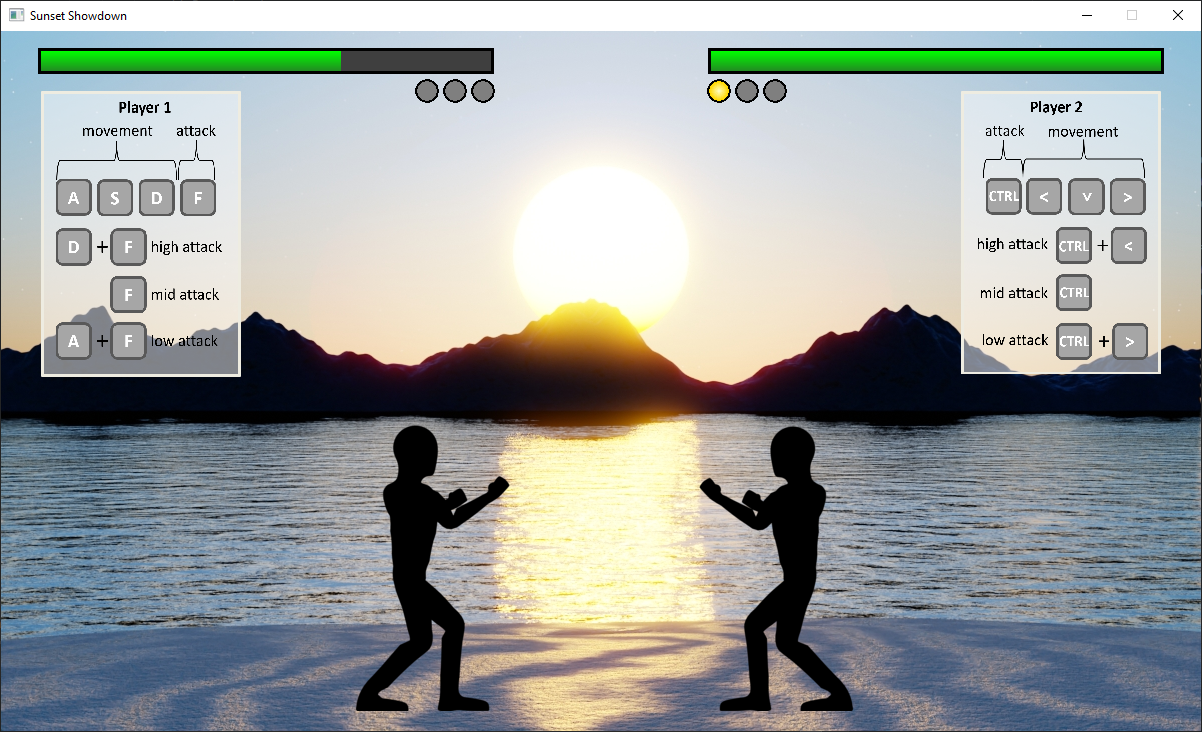
\includegraphics[width=0.64\linewidth]{rys02/interfejs}
	\caption{Zrzut ekranu z gry Sunset Showdown z widocznym interfejsem gry}
	\label{fig:interfejs}
\end{figure}
Na rysunku \ref{fig:interfejs} widoczny jest interfejs użytkownika gry Sunset Showdown. Postacie graczy są zaprezentowane jako sylwetki w jednolitym, czarnym kolorze. W górnej części ekranu umieszczone są zielone paski zdrowia dla każdego z graczy, które zmniejszają się w miarę otrzymywania obrażeń przez postacie. Poniżej pasków zdrowia znajdują się ikony w kształcie kółek, które jeżeli zapalone na żółto wskazują na wygrane rundy.

Po bokach ekranu umiejscowione są schematy sterowania dla każdego z graczy, przedstawiające przypisane klawisze i ich funkcje w grze. Dla Gracza 1, po lewej stronie, przyciski 'A', 'S', 'D', i 'F' odpowiadają za ruchy i podstawowe ataki, z dodatkowymi kombinacjami klawiszy dla ataków wysokich, średnich i niskich. Analogicznie, Gracz 2, po prawej stronie ekranu, korzysta z klawiszy strzałek oraz 'CTRL' do sterowania swoją postacią i wykonania ataków.

\section{Tryby gry}
W "Sunset Showdown" dostępne będą dwa podstawowe tryby gry. Tryb offline umożliwi dwóm graczom wspólną rozgrywkę na jednym komputerze przy użyciu tej samej klawiatury. Oprócz tego, gra będzie oferować tryb online, który pozwala graczom na połączenie się przez internet z osobnych komputerów. W tym trybie gracze będą mogli tworzyć pokoje gry, do których dostęp jest możliwy po wprowadzeniu specjalnego kodu pokoju. Aby założyć pokój, niezbędne będzie połączenie komputera do routera z aktywną opcją Universal Plug and Play (UPnP). Natomiast dołączenie do pokoju będzie wymagało jedynie standardowego połączenia internetowego. Funkcjonalności te będą dostępne w menu głównym gry.
\chapter{Implementacja}
W niniejszym rozdziale przedstawiono szczegółową analizę implementacji dwuwymiarowej gry zręcznościowej z gatunku bijatyk. Omówienie obejmuje kluczowe aspekty techniczne projektu, takie jak tworzenie animacji, struktura klas, wzorce projektowe oraz implementacja mechanik gry, zarówno w trybie offline, jak i online. Szczególny nacisk położono na takie elementy, jak zarządzanie postaciami, detekcja kolizji, obsługa sieci oraz interfejs użytkownika, które razem stanowią rdzeń funkcjonalności i grywalności projektu.
\section{Tworzenie animacji}
\begin{figure}
	\centering
		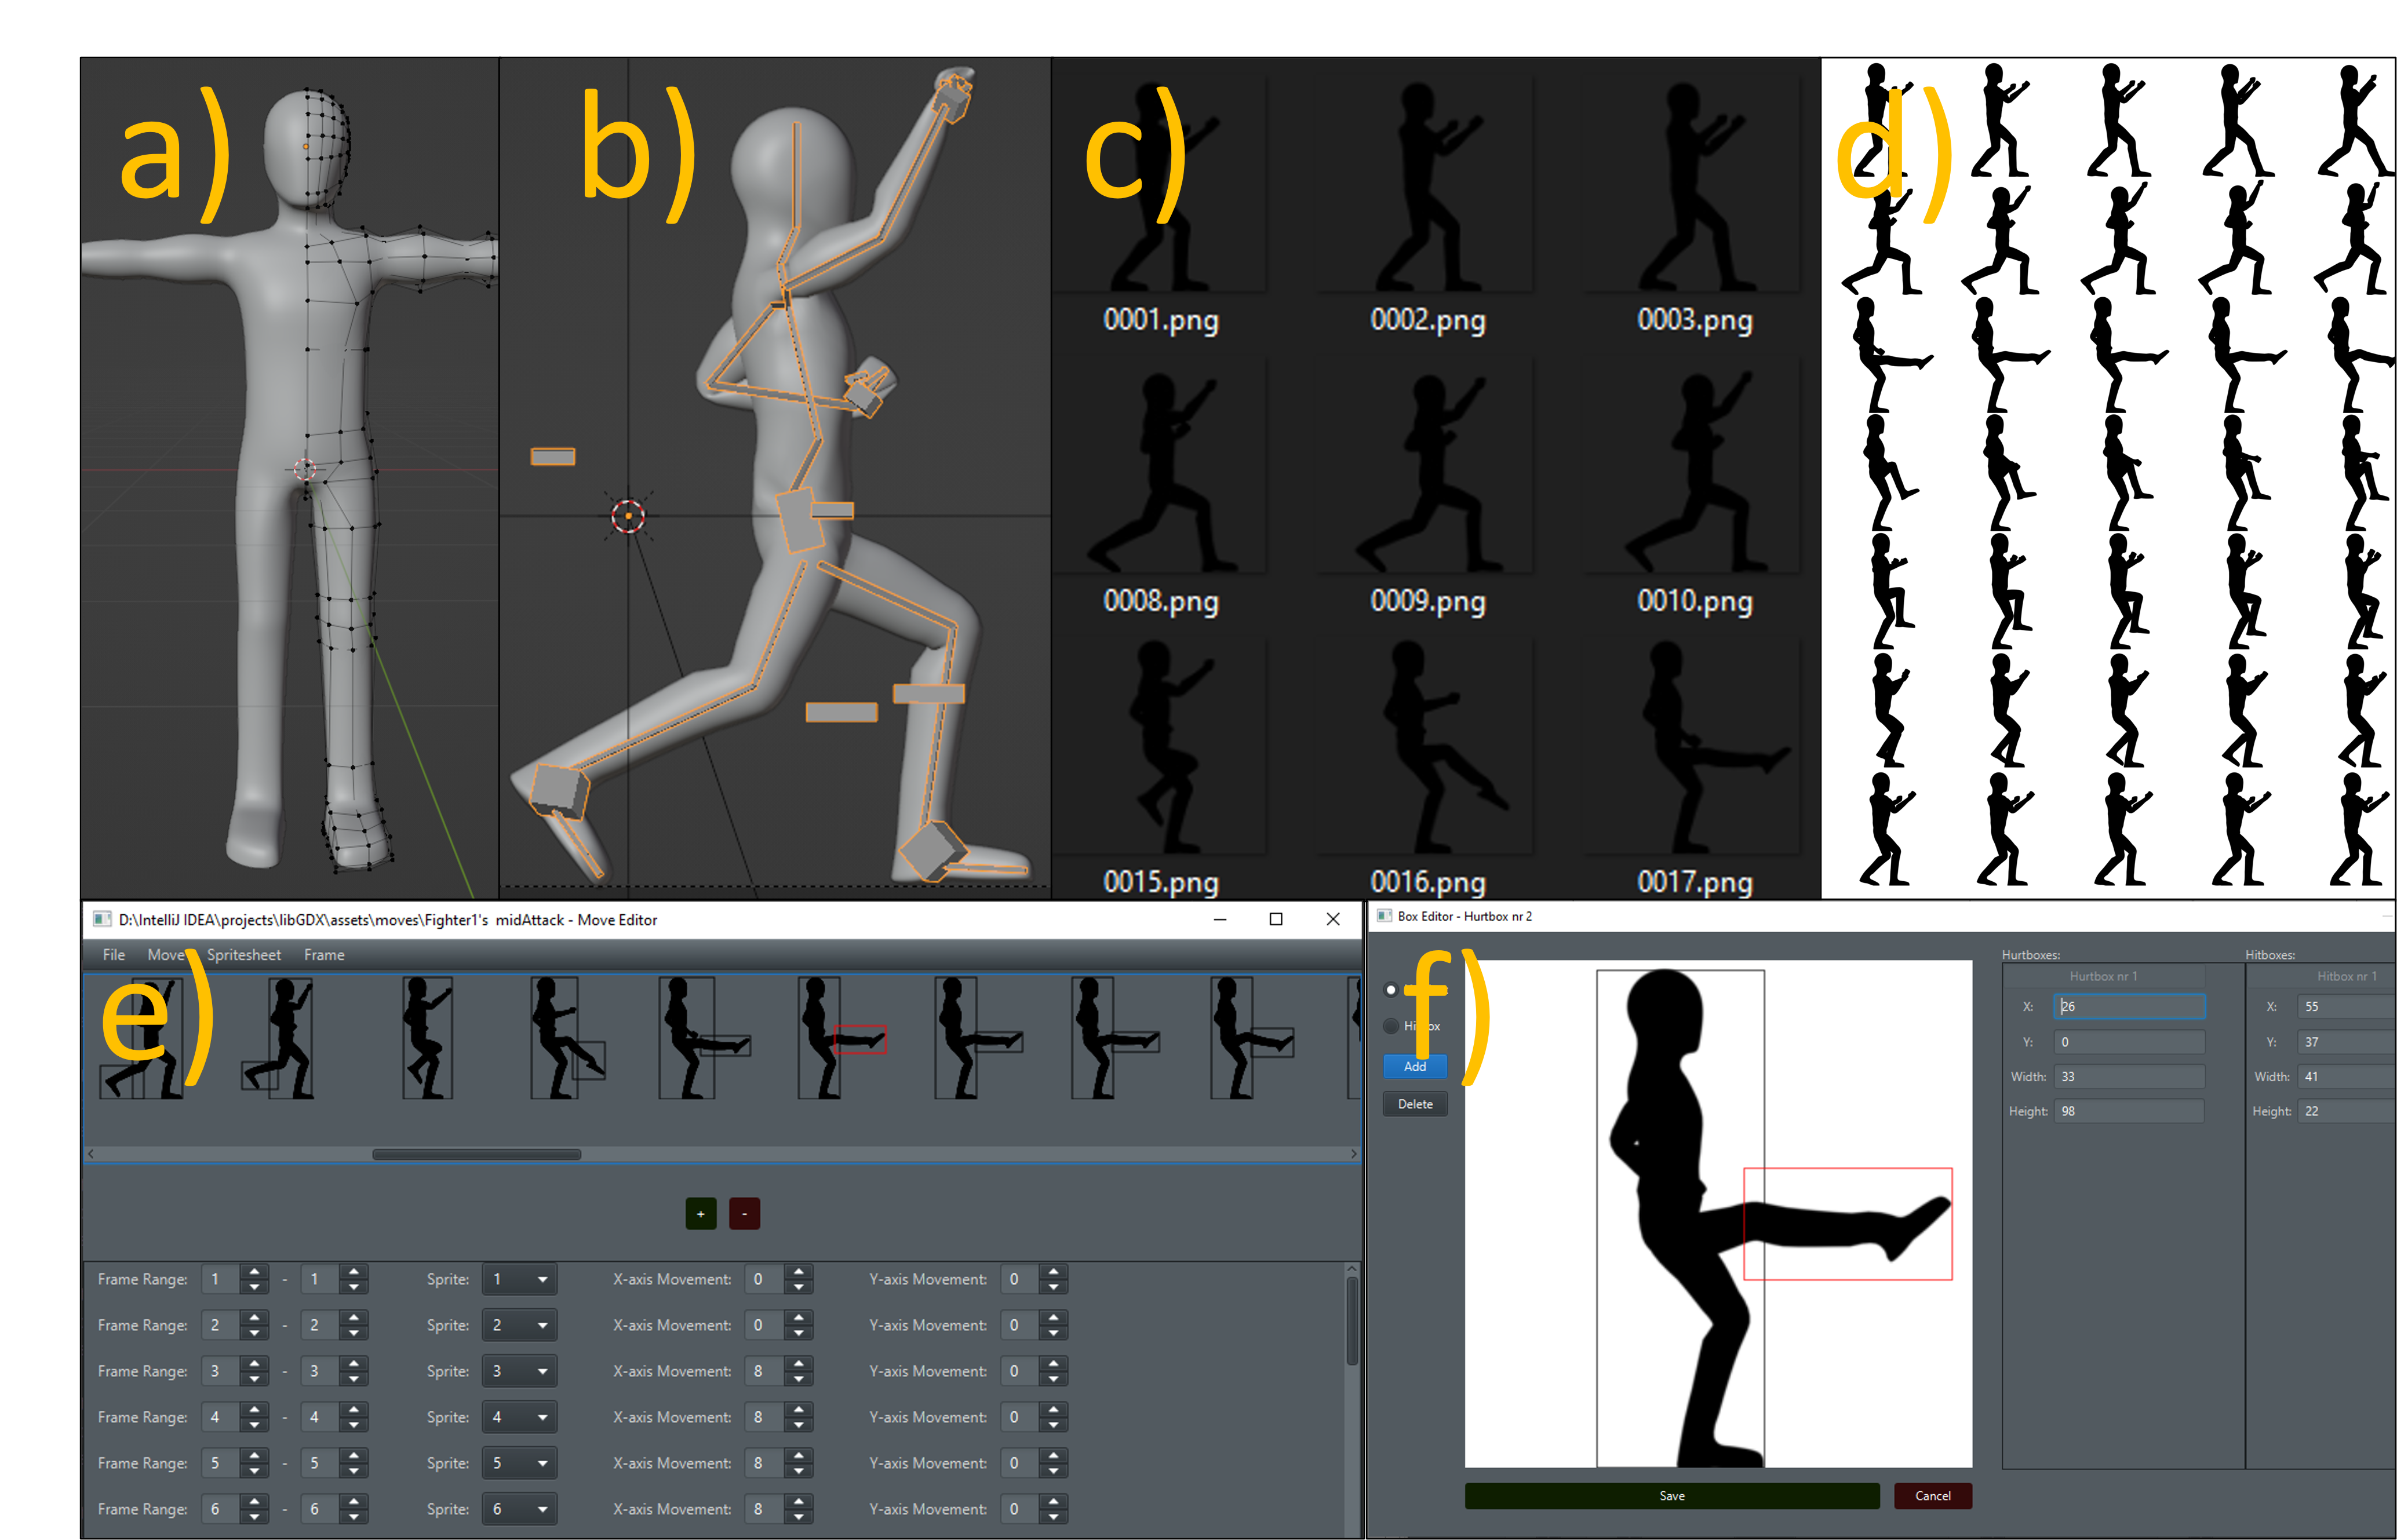
\includegraphics[width=0.64\linewidth]{rys03/animacja}
	\caption{Proces tworzenia animacji}
	\label{fig:animacja}
\end{figure}
Na rysunku \ref{fig:animacja} pokazano proces tworzenia animacji. a) Na początku postać została zamodelowana w 3D. Użyto do tego narzędzia Blender. b) Następnie przeprowadzono \emph{rigging}, czyli proces dodawania szkieletu do modelu 3D, który pozwala na animowanie poszczególnych części ciała. c) Po ustawieniu postaci w pożądanych pozach, każda klatka animacji była renderowana i zapisywana jako seria oddzielnych plików graficznych (\emph{sprite'ów}). Te obrazy stanowiły podstawę dla każdego ruchu postaci w grze. d) Następnie używając narzędzia ImageMagick \emph{sprite'y} zostały połączone w jeden większy obraz zwany \emph{spritesheet'em}. e) Używając stworzonego przez autora pracy, na potrzeby tego projektu, narzędzia do edycji animacji \emph{Move Editor}, stworzono wpisy do każdej klatki, opisujące między innymi ruch postaci. f) W Move Editorze określano również \emph{hurtbox'y} i \emph{hitbox'y} dla każdej klatki animacji. \emph{Hurtbox} to obszar, w którym postać może otrzymać obrażenia, natomiast \emph{hitbox} to obszar, w którym postać zadaje obrażenia. Ta funkcjonalność jest kluczowa dla mechaniki gry, ponieważ decyduje o tym, kiedy ataki postaci trafiają lub są blokowane. Po zakończeniu edycji \emph{spritesheet} wraz z opisem klatek w formacie json zostały zapisane w odpowiedniej strukturze plików, aby mogły być bezpośrednio wykorzystane w grze.
% TO DO: a czy nie dałoby się stworzyć rysunku z białym tłem? Czarne tło źle wygląda na wydrukach.
\section{Struktura klas}
Na rysunku \ref{fig:struktura_klas} przedstawiono główne klasy stworzone na potrzeby gry. W poniższych podsekcjach zamieszczono krótki opis każdej z nich.
\begin{figure}[htb]
	\centering
		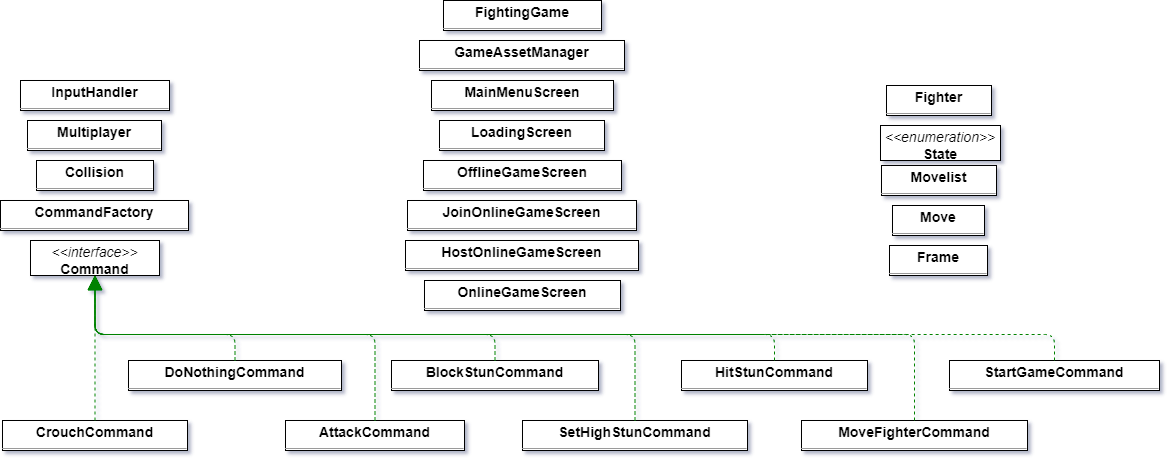
\includegraphics[width=1\linewidth]{rys03/struktura_klas}
	\caption{Struktura zaprojektowanych klas}
	\label{fig:struktura_klas}
\end{figure}

\subsection{Główna struktura gry}
\texttt{FightingGame} służy jako centrum zarządzania głównymi aspektami gry, takimi jak inicjalizacja, cykl życia gry oraz przełączanie pomiędzy różnymi ekranami (np. menu, gra itp.). W procesie inicjalizacji wykorzystuje klasę \texttt{GameAssetManager}, która odpowiada za wczytywanie i zarządzanie zasobami gry, takimi jak tekstury, dźwięki i~inne elementy multimedialne.

\texttt{MainMenuScreen}, \texttt{LoadingScreen}, \texttt{OfflineGameScreen}, \texttt{JoinOnlineGameScreen}, \texttt{HostOnlineGameScreen} oraz \texttt{OnlineGameScreen} są klasami reprezentującymi różne ekrany w grze, każdy z nich implementuje interfejs \texttt{Screen} dostarczony przez framework \texttt{libGDX}. Zapewniają one różnorodne interfejsy uzytkownika i są odpowiedzialne za prezentację odpowiedniego widoku w zależności od stanu gry.

\subsection{Mechanika rozgrywki}
Klasa \texttt{Fighter} reprezentuje postać walczącą. Przechowuje ona wartości takie jak zdrowie, pozycję, \emph{hurtbox'y} i \emph{hitbox'y} postaci oraz stan w którym aktualnie się znajduje. Ten stan reprezentowany jest przez typ wyliczeniowy \texttt{State} i obejmuje takie sytuacje jak ,,chodzenie do przodu'', ,,cofanie się'', ,,kucanie'' jak i wykonywanie różnych ataków albo otrzymywanie ich na bloku lub bez niego. Na podstawie tej klasy często wykonuje się logika reszty programu. 

Awatar, którym steruje gracz, posiada zestaw ruchów zawarty w klasie \texttt{Movelist}. Ta klasa przetrzymuje poszczególne ruchy o klasie \texttt{Move}. Każdy cios jest opisany poprzez pojedyncze klatki za pomocą klasy \texttt{Frame}, w których znajduje się informacja o ruchu jaki postać ma wykonać, jaki zestaw obszarów określających kolizję ma mieć wpływ na postać w danym momencie oraz jaki \texttt{sprite} ma zostać wyświetlony.

\subsection{Wykrywanie kolizji, obsługa wejścia i wzorzec \emph{command} \cite{GPP}}
Klasy \texttt{Command}, \texttt{CommandFactory}, \texttt{DoNothingCommand}, \texttt{BlockStunCommand}, \texttt{HitStunCommand}, \texttt{SetHighStunCommand}, \texttt{MoveFighterCommand}, \texttt{StartGameCommand} wdrażają wzorzec programowania \emph{command} (polecenia), umożliwiając abstrakcyjne reprezentacje akcji, które mogą być wykonane w grze. \texttt{Command} jest interfejsem dla wszystkich komend, \texttt{CommandFactory} jest fabryką do tworzenia instancji komend, a pozostałe klasy są konkretnymi komendami, które mogą być wywołane przez graczy lub system gry. Klasa \texttt{InputHandler} zajmuje się obsługą wejścia od użytkownika - tworzy komendy na podstawie przycisku naciśniętego przez gracza oraz aktualnego stanu postaci. \texttt{Collision} zarządza detekcją kolizji między postaciami w grze oraz wpływa na stan tych postaci. \texttt{Multiplayer} odpowiada za implementację funkcjonalności sieciowych, umożliwiając grę wieloosobową poprzez zarządzanie połączeniami i komunikacją między graczami. Gdy postać jest sterowana przez gracza połączonego przez internet to właśnie ta klasa podaje komendy do wykonania przez jego awatar wpływając na działanie \texttt{InputHandler'a}.

\section{Fragmenty kodu}
W tej sekcji zostaną omówione fragmenty kodu, które zostały uznane przez autora pracy inżynierskiej za kluczowe w działaniu programu.
\subsection{Interfejs \texttt{Command}}
Na listingu \ref{list:command} zaprezentowano interfejs, który jest implementowany przez wiele innych klas. Interfejs ten nakazuje implementującym go klasom stworzenie metody \texttt{execute}, która najczęściej zmieniać ma stan jakiegoś obiektu (np.\ z klasy \texttt{Fighter}) oraz metody \texttt{undo}, mającej za zadanie wycofanie zmian wprowadzonych metodą \texttt{execute}. Dzięki temu podejściu można na przykład łatwo zmieniać przypisane do przycisków zadania lub stworzyć historię wciśniętych przycisków, a także system powtórek bazujących na logice \emph{undo}. Dodatkowo, tworzenie obiektów reprezentujących wykonywane akcje ułatwia proces tworzenia kodu sieciowego.
\begin{lstlisting}[language=Java,style=JavaStyle,label=list:command,caption=Interfejs \texttt{Command},
                   basicstyle=\footnotesize\ttfamily]
public interface Command {
    void execute(Entity entity);
    void undo(Entity entity);
}
\end{lstlisting}

\subsection{Klasa \texttt{Fighter}}
Klasa \texttt{Fighter} zarządza stanem i zachowaniem postaci w grze. Zawiera informacje o zdrowiu, listy obszarów trafień (\emph{hitboxes}) i obszarów, które mogą zostać trafione (\emph{hurtboxes}), oraz zestaw ruchów (\emph{movelist}). Wykorzystuje ona wzorzec programowania \emph{update}. Sprowadza się on do implementacji metody aktualizacji stanu, która symuluje jedną klatkę zachowania obiektu. Na listingu \ref{list:fighter} można zauważyć, że metoda ta tworzy rozkaz za pomocą klasy \texttt{InputHandler}, a~następnie wykonuje go. W kolejnym kroku, jeżeli gracz uczestniczy w rozgrywce online, jego komenda jest przesyłana do drugiego gracza z pomocą klasy \texttt{Multiplayer}. Na końcu postać w grze aktualizuje wyświetlany \texttt{sprite} oraz inne informacje dotyczące aktualnej klatki animacji.

\begin{lstlisting}[language=Java,style=JavaStyle,label=list:fighter,caption=Funkcja update w klasie Fighter,
                   basicstyle=\footnotesize\ttfamily]
public void update() {
    Command command = inputHandler.handleInput();
    command.execute(this);
    if (multiplayer != null && (player == Player.PLAYER1 || player == Player.PLAYER2)) {
        multiplayer.sendCommand(command);
    }
    updateAnimation();
}
\end{lstlisting}

\subsection{Klasa \texttt{OfflineGameScreen}}
Listing \ref{list:offline_game} przedstawia implementację klasy \texttt{OfflineGameScreen}. Klasa ta wykorzystuje wzorzec pętli gry (\emph{game loop pattern}), wraz z wzorcem aktualizacji (\emph{update pattern}), aby zarządzać cyklem życia gry w trybie \emph{offline}. Konstruktor inicjalizuje stan gry, przydzielając graczy i tworząc kolekcję bytów (\texttt{entities}), które będą aktualizowane i renderowane w każdym cyklu gry. Inicjalizuje również system kolizji, który jest odpowiedzialny za wykrywanie i rozwiązywanie interakcji między bytami. Klasa implementuje interfejs \texttt{Screen} z frameworka \texttt{LibGDX}, co oznacza, że musi dostarczyć implementację metody \texttt{render}, która jest wywoływana na każdą klatkę gry. Ta metoda jest rdzeniem pętli gry. Przyjmuje parametr \texttt{delta}, który reprezentuje czas, jaki upłynął od ostatniej klatki, umożliwiając aktualizacje oparte na czasie rzeczywistym. Na początku każdej klatki ekran jest czyszczony. 

Metoda \texttt{updateEntities} jest wywoływana w celu zaktualizowania stanu wszystkich bytów w grze. Zawiera logikę warunkową, która decyduje, czy byty powinny być aktualizowane w stanie bezczynności (\texttt{idle}), po zakończeniu rundy (\texttt{updateRoundEnd}), czy w standardowym trybie gry, gdzie każdy byt jest aktualizowany poprzez wywołanie jego metody update. Te dwie pierwsze są oddzielone od standardowego trybu ze względu na to że w trybie online będą one mogły wykonywać się po stronie klienta, niezależnie od przychodzących przez internet informacji od drugiego gracza. Po zaktualizowaniu bytów, system kolizji jest aktualizowany, aby sprawdzić i przetworzyć wszelkie kolizje, które miały miejsce pomiędzy bytami. 

Na koniec metoda \texttt{renderGame} odpowiada za narysowanie aktualnego stanu gry na ekranie.

\begin{lstlisting}[language=Java,style=JavaStyle,label=list:offline_game,caption=Klasa \texttt{OfflineGameScreen},
                   basicstyle=\footnotesize\ttfamily]
public class OfflineGameScreen implements Screen {
    FightingGame game;
    private Collection<Entity> entities;
    private Collision collision;
    ...// Pozostałe tekstury, dźwięki itp

    public OfflineGameScreen(FightingGame game) {
        // Przydzielanie graczy
        game.player1.setPlayer(Player.PLAYER1);
        game.player2.setPlayer(Player.PLAYER2);

        // Inicjalizacja kolekcji bytów i kolizji
        entities = new ArrayList<>();
        entities.add(game.player1);
        entities.add(game.player2);
        collision = new Collision(game.player1, game.player2); 
        ...// Pobieranie załadowanych zasobów za pomocą AssetManagera
    }

    @Override
    public void render(float delta) {
        ...
        //clear
        clearScreen();
        //update
        updateEntities();
        //render
        renderGame();
		...
    }
		
		private void updateEntities() {
        if (isCountdownActive || isFightMessageActive) {
            game.player1.updateIdle();
            game.player2.updateIdle();
        } else if (isWinnerMessageActive) {
            game.player1.updateRoundEnd();
            game.player2.updateRoundEnd();
        } else {
            for (Entity entity : entities) {
                entity.update();
            }
            collision.update();
        }
    }
		...
}
\end{lstlisting}

\subsection{Klasa \texttt{Multiplayer}}
Klasa \texttt{Multiplayer} została stworzona w celu obsługi połączenia między graczami w trybie online. Wykorzystuje ona biblioteki kryo \cite{Kryo}, kryonet \cite{Kryonet} oraz weupnp \cite{weupnp}, co jest widoczne w importach klasy w listingu \ref{list:multiplayer}. Konstruktor klasy nie otwiera jeszcze żadnego połączenia, a konkretne metody obsługi połączenia są wywoływane dopiero po wybraniu przez użytkownika odpowiedniego trybu gry. 
Jeśli gracz wybierze opcję hostowania meczu, oznacza to uruchomienie serwera na jego komputerze za pomocą funkcji \texttt{initializeServer}. Funkcja ta rozpoczyna od znalezienia wolnego portu, którym domyślnie jest port 54555. Następnie próbuje otworzyć go za pomocą funkcji \texttt{openPortUPnP}, która wyszukuje dostępny router i sprawdza jego zewnętrzny adres IP, a następnie tworzy mapowanie portów. Po tych krokach tworzony jest serwer i przypisywane są do niego klasy do serializacji i deserializacji. Serwer nasłuchuje różne zdarzenia, takie jak połączenie i rozłączenie drugiego gracza, które zmieniają flagi klasy \texttt{Multiplayer}. Dodatkowo, jeśli do serwera przyjdzie instancja obiektu \texttt{Command} jest ona dodawana do kolejki komend. Na podstawie tej kolejki \texttt{InputHandler} definiuje zachowanie postaci gracza połączonego przez sieć. Ostatecznie serwer jest przypisywany do portu, na którym ma pracować. 
W przypadku wyboru przez użytkownika opcji dołączenia do pokoju i podania kodu uzyskanego od drugiego gracza, uruchamiana jest funkcja \texttt{initializeClient}. Podobnie jak w przypadku serwera, klient również nasłuchuje przychodzące wiadomości. Jedyną różnicą jest obsługa konkretnych komend, takich jak rozpoczęcie gry czy wiadomość o powaleniu przeciwnika. Reszta komend jest obsługiwana w podobny sposób jak na serwerze. 
Klasa \texttt{Multiplayer} posiada także funkcje do zamykania serwera i klienta \texttt{closeServer} i \texttt{closeClient}, które służą do zakończenie połączenia po zakończeniu rozgrywki i w przypadku serwera również zakończenie przekierowania portów na routerze.

\begin{lstlisting}[language=Java,style=JavaStyle,label=list:multiplayer,caption=Klasa \texttt{Multiplayer},
                   basicstyle=\footnotesize\ttfamily]
package com.mygdx.game;

import com.esotericsoftware.kryo.Kryo;
import com.esotericsoftware.kryonet.Connection;
import com.esotericsoftware.kryonet.Listener;
import com.esotericsoftware.kryonet.Server;
import com.esotericsoftware.kryonet.Client;
...
import org.bitlet.weupnp.GatewayDevice;
import org.bitlet.weupnp.GatewayDiscover;
import org.bitlet.weupnp.PortMappingEntry;


public class Multiplayer {
    private Server server;
    private Client client;
    private int serverPort;
    private int connectedPort;
    private boolean isAttemptingConnection = false;
    private boolean isConnected = false;
    private boolean startGame = false;
    private String lastErrorMessage = null;
	...
    String ipAddress;
    LinkedBlockingDeque<Command> commandQueue;

    public Multiplayer() {
        this.commandQueue = new LinkedBlockingDeque<>();
    }

    public void initializeServer() {
        isAttemptingConnection = true;
        serverPort = findFreePort();
        if (openPortUPnP(serverPort)) {
            System.out.println("UPnP: Port został otwarty");
        } else {
            System.out.println("UPnP: Nie udało się otworzyć portu, sprawdź konfigurację routera lub ustawienia firewalla");
        }
        server = new Server();
        client = null;
        configureKryo(server.getKryo());

        server.addListener(new Listener() {
            @Override
            public void connected(Connection connection) {
                isConnected = true;
                lastErrorMessage = null;
            }
            @Override
            public void received(Connection connection, Object object) {
                if (object instanceof Command) {
                    System.out.println("received: " + object);
                    handleCommand((Command) object);
                }
            }
            @Override
            public void disconnected(Connection connection) {
                isConnected = false;
                lastErrorMessage = "Disconnected";
            }
        });

        ipAddress = getPublicIpAddress();
        System.out.println("IpAddress: " + ipAddress);
        try {
            server.bind(serverPort);
            server.start();
            System.out.println(" Server started on serverPort: " + serverPort);
        } catch (IOException e) {
            lastErrorMessage = "Connection error: " + e.getMessage();
            e.printStackTrace();
        }
    }

    public void closeServer() {
        if (server != null) {
            server.stop();
            server = null;
            removePortUPnP(serverPort);
            System.out.println("Serwer zostal zamkniety.");
        }
    }


    public void initializeClient(String ipAddress, int port) {
        isAttemptingConnection = true;
        client = new Client();
        configureKryo(client.getKryo());

        client.addListener(new Listener() {
            @Override
            public void connected(Connection connection) {
                isConnected = true;
                lastErrorMessage = null;
            }
            @Override
            public void received(Connection connection, Object object) {
                if (object instanceof SetHighStunCommand) {
                    System.out.println("received: " + object);
                    player1IsHitStunned = true;
                }
                else if (object instanceof StartGameCommand) {
                    startGame = true;
                } else if (object instanceof Command) {
                    System.out.println("received: " + object);
                    handleCommand((Command) object);
                }
            }
            @Override
            public void disconnected(Connection connection) {
                isConnected = false;
                lastErrorMessage = "disconnected";
            }
        });

        try {
            client.start();
            //System.out.println("Klient probuje sie polaczyc z " + ipAddress + "/" + port);
            client.connect(5000, ipAddress, port);
            this.ipAddress = ipAddress;
        } catch (IOException e) {
            lastErrorMessage = "Connection error: " + e.getMessage();
            e.printStackTrace();
        }
    }

    public void closeClient() {
        if (client != null) {
            client.stop();
            client = null;
            System.out.println("Klient zostal zamkniety.");
        }
    }

    public void stopServer() {
        if (server != null) {
            // Usuń mapowanie portów za pomocą UPnP
            removePortUPnP(serverPort);
            server.stop();
            server.close();
            System.out.println("Serwer zatrzymany");
        }
    }

    private void handleCommand(Command command) {
        commandQueue.add(command);
    }

    public void sendCommand(Command command) {
        if (server != null) {
            System.out.println("send: " + command);
            server.sendToAllTCP(command);
        } else if (client != null) {
            System.out.println("send: " + command);
            client.sendTCP(command);
        }

    }

    public boolean openPortUPnP(int port) {
        try {
            GatewayDiscover discover = new GatewayDiscover();
            discover.discover();
            GatewayDevice d = discover.getValidGateway();

            if (d == null) {
                System.out.println("Nie znaleziono bramy UPnP!");
                return false;
            }

            System.out.println("Znaleziono brame UPnP: " + d.getModelName());

            // Pobierz zewnętrzny adres IP
            String externalIPAddress = d.getExternalIPAddress();
            System.out.println("Zewnetrzny adres IP to: " + externalIPAddress);

            // Utwórz mapowanie portów
            boolean done = d.addPortMapping(port, port, d.getLocalAddress().getHostAddress(), "TCP", "KryoNet Game Server");

            if (done) {
                System.out.println("Port przekierowany: " + port);
                return true;
            } else {
                System.out.println("Nie udalo się przekierować portu: " + port);
                return false;
            }
        } catch (Exception e) {
            e.printStackTrace();
            return false;
        }
    }

    public boolean removePortUPnP(int port) {
        try {
            GatewayDiscover discover = new GatewayDiscover();
            discover.discover();
            GatewayDevice d = discover.getValidGateway();
            if (d != null) {
                return d.deletePortMapping(port, "TCP");
            }
        } catch (Exception e) {
            e.printStackTrace();
        }
        return false;
    }
		...
}
									
\end{lstlisting}
\chapter{Testy}
Ten rozdział poświęcony jest prezentacji testów przeprowadzonych w ramach projektu. Testy automatyczne zostały przeprowadzone z użyciem JUnit \cite{JUnit} i Mockito \cite{Mockito}.

\section{Testy automatyczne}
\subsection{\texttt{FighterTest}}
W celu zweryfikowania poprawnego działania klasy \texttt{Fighter} napisano i przeprowadzono test sprawdzający działanie metody \texttt{update} (metoda ta zajmuje się aktualizacją stanu obiektu w każdej klatce). Implementacja testu zaczyna się od zaimportowania wszystkich potrzebnych komponentów (patrz listing \ref{list:FighterTest}). W funkcji \texttt{init}, która jest udekorowana adnotacją \texttt{@BeforeAll}, zawarte są wszystkie potrzebne inicjalizacje związane z frameworkiem \texttt{LibGDX} oraz jego uruchomieniem bez środowiska graficznego. Następnie w funkcji \texttt{setUp} tworzone są wszystkie potrzebne obiekty do testów -- obiekt klasy \texttt{Fighter} oraz \texttt{GameAssetManager}. 

Sam test miał sprawdzać, czy poprawnie zmienia się stan obiektu z klasy \texttt{Fighter}. Dlatego należało zasymulować wciśnięcie przycisku, a dokładniej -- zwrócenie odpowiedniego polecenia z metody \texttt{handleInput} instancji obiektu "InputHandler". W teście takie \emph{mockowanie} zrealizowane jest poprzez zwracanie komendy \emph{MoveFighterCommand} jeżeli wywołana zostanie funkcja \texttt{handleInput}.

Test rozpoczyna się od potwierdzenia stanu dopiero utworzonej postaci. Następnie wywoływana jest funkcja \texttt{update}, która ma za zadanie zaktualizować postać na podstawie komendy. Następnie sprawdzane jest czy prawidłowo zmienione zostały konkretne pola. Dokładniej mówiąc sprawdzane jest czy postać dopiero rozpoczyna animację (czy znajduje się w klatce o zerowym indeksie), czy poruszyła się o odpowiednią odległość, czy jej stan został odpowiednio zmieniony, czy obszary kolizji zmieniły się na te zgodne z aktualną animacją oraz czy podmieniona została wyświetlana aktualnie tekstura. 

Test przebiegł pomyślnie potwierdzając wszystkie sprawdzenia.
\begin{lstlisting}[language=Java,style=JavaStyle,label=list:FighterTest,caption=Test metody \texttt{update} z klasy \texttt{Fighter},
                   basicstyle=\footnotesize\ttfamily]
							
package com.mygdx.entities;
...
import static org.junit.jupiter.api.Assertions.assertEquals;
import static org.mockito.Mockito.mock;
import static org.mockito.Mockito.when;

public class FighterTest extends ApplicationAdapter {
    private Fighter fighter;
    private InputHandler mockInputHandler;
    private int initialX, initialY;

    @BeforeAll
    public static void init() {
        HeadlessApplicationConfiguration conf = new HeadlessApplicationConfiguration();
        new HeadlessApplication(new FightingGame(), conf);
        Gdx.gl = mock(GL20.class);
        Gdx.gl20 = mock(GL20.class);
    }
    @BeforeEach
    void setUp() {
        initialX = 0;
        initialY = 0;
        mockInputHandler = mock(InputHandler.class);
        GameAssetManager gameAssetManager = new GameAssetManager();
        gameAssetManager.loadAssets();
        while (!gameAssetManager.manager.update()) {
            // oczekiwanie aż wszystkie zasoby sie załadują
        }
        fighter = new Fighter(initialX, initialY, Player.PLAYER1, 0, 0, 0, 0, 10, gameAssetManager.manager);
        fighter.setInputHandler(mockInputHandler);
    }

    @Test
    void testUpdateWithMoveForwardCommand() {
        // Sprawdzenie początkowego stanu postaci
        assertEquals(0, fighter.getCurrentFrame());
        assertEquals(initialX, fighter.getX());
        assertEquals(initialY, fighter.getY());
        assertEquals(State.NEUTRAL, fighter.getState());
        Move idleMove = fighter.getMovelist().getMove(State.NEUTRAL.getId());
        List<Rectangle> initialHurtboxes = idleMove.getFrame(0).getHurtboxes();
        List<Rectangle> initialHitboxes = idleMove.getFrame(0).getHitboxes();
        TextureRegion initialSprite = idleMove.getFrame(0).getSprite();
        assertEquals(initialHurtboxes, fighter.getHurtboxes());
        assertEquals(initialHitboxes, fighter.getHitboxes());
        assertEquals(initialSprite, fighter.getTextureRegion());

        // Symulacja otrzymania komendy MoveFighterCommand od InputHandler'a
        when(mockInputHandler.handleInput()).thenReturn(CommandFactory.moveFighterCommandForward(fighter));

        // Aktualizacja logiki postaci
        fighter.update();

        // Sprawdzenie, czy aktualna klatka animacji to 0
        assertEquals(0, fighter.getCurrentFrame());

        // Sprawdzenie, czy postać poruszyła się o oczekiwaną odległość
        Move goingForwardMove = fighter.getMovelist().getMove(State.GOING_FORWARD.getId());
        int xAxisMovement = goingForwardMove.getFrame(0).getXAxisMovement();
        int yAxisMovement = goingForwardMove.getFrame(0).getYAxisMovement();
        assertEquals(initialX + xAxisMovement, fighter.getX());
        assertEquals(initialY + yAxisMovement, fighter.getY());

        // Sprawdzenie, czy stan postaci zmienił się na GOING_FORWARD
        assertEquals(State.GOING_FORWARD, fighter.getState());

        // Sprawdzenie, czy hurtboxy i hitboxy są zgodne z aktualną klatką ruchu
        List<Rectangle> hurtboxes = goingForwardMove.getFrame(0).getHurtboxes();
        for (Rectangle hurtbox : hurtboxes) {
            // Jako że położenie hurtboxów jest względne (wobec postaci)
            // to należy jeszcze dodać przebytą drogę
            hurtbox.x = hurtbox.x + xAxisMovement;
        }
        List<Rectangle> hitboxes = goingForwardMove.getFrame(0).getHitboxes();
        for (Rectangle hitbox : hitboxes) {
            // Jako że położenie hitboxów jest względne (wobec postaci)
            // to należy jeszcze dodać przebytą drogę
            hitbox.x = hitbox.x + xAxisMovement;
        }
        assertEquals(hurtboxes ,fighter.getHurtboxes());
        assertEquals(hitboxes ,fighter.getHitboxes());

        // Sprawdzenie czy postac zmienilła wyświetlaną teksturę
        TextureRegion sprite = goingForwardMove.getFrame(0).getSprite();
        assertEquals(sprite, fighter.getTextureRegion());
    }
}
\end{lstlisting}

\subsection{\texttt{CollisionTest}}
Test polega na symulowaniu serii klatek gry, w których atakujący wykonuje atak wysoki (high attack), a odbierający porusza się do przodu. Celem jest sprawdzenie, czy w odpowiedniej klatce dochodzi do kolizji i czy system poprawnie reaguje na tę sytuację, zmieniając stan postaci odbierającej na \texttt{HIT\_STUNNED\_HIGH} oraz czy poprawnie odejmuje jej zdrowie.

\begin{lstlisting}[language=Java,style=JavaStyle,label=list:CollisionTest,caption=Test poprawnego wykrywania kolizji w klasie \texttt{Collision},
                   basicstyle=\footnotesize\ttfamily]
package com.mygdx.engine;
...
import static org.junit.jupiter.api.Assertions.*;
import static org.mockito.Mockito.*;

public class CollisionTest extends ApplicationAdapter {
    Collision collision;
    private Fighter attacker, receiver;
    private InputHandler attackerMockInputHandler, receiverMockInputHandler;
    private int attackerInitialX, attackerInitialY, receiverInitialX, receiverInitialY;
    @BeforeAll
    public static void init() {
        HeadlessApplicationConfiguration conf = new HeadlessApplicationConfiguration();
        new HeadlessApplication(new FightingGame(), conf);
        Gdx.gl = mock(GL20.class);
        Gdx.gl20 = mock(GL20.class);
    }
    @BeforeEach
    void setUp() {
        // Początkowe rozmieszczenie umieszcza postacie tuż obok siebie
        attackerInitialX = 0;
        attackerInitialY = 0;
        receiverInitialX = 300;
        receiverInitialY = 0;
        GameAssetManager gameAssetManager = new GameAssetManager();
        gameAssetManager.loadAssets();
        while (!gameAssetManager.manager.update()) {
            // oczekiwanie aż wszystkie zasoby sie zaladują
        }
        attacker = new Fighter(attackerInitialX, attackerInitialY, Player.PLAYER1, 0, 0, 0, 0, 10, gameAssetManager.manager);
        attackerMockInputHandler = spy(new InputHandler(attacker, Player.PLAYER1, 0, 0, 0, 0, 10));
        attacker.setInputHandler(attackerMockInputHandler);
        receiver = new Fighter(receiverInitialX, receiverInitialY, Player.PLAYER2, 0, 0, 0, 0, 10, gameAssetManager.manager);
        receiverMockInputHandler = spy(new InputHandler(receiver, Player.PLAYER2, 0, 0, 0, 0, 10));
        receiver.setInputHandler(receiverMockInputHandler);
        collision = new Collision(attacker, receiver);
    }

    @Test
    void testCollisionDetectionAndAftermaths() {
        // Symulacja otrzymania komendy AttackCommand od InputHandler'a
        doAnswer(invocation -> {
            Command command = CommandFactory.AttackCommandHigh(attacker);
            attackerMockInputHandler.getCommandHistory().add(command);
            attacker.setCurrentFrame(attacker.getCurrentFrame() + 1);
            return command;
        }).when(attackerMockInputHandler).handleInput();
        // Symulacja funkcjonalności InputHandler.handleInput() ograniczającej się
        // do zwracania komendy MoveFighterCommand lub HitStunCommand w przypadku,
        // gdy Collision wykryje otrzymanie ataku high
        doAnswer(invocation -> {
            Command command = CommandFactory.moveFighterCommandForward(receiver);
            int currentFrame = receiver.getCurrentFrame() + 1;
            if (receiver.isHitStunnedHigh()) {
                if (receiver.getState() != State.HIT_STUNNED_HIGH) {
                    receiver.setCurrentFrame(0);
                    command = CommandFactory.hitStunCommandHigh(receiver);
                    receiverMockInputHandler.getCommandHistory().add(command);
                    return command;
                } else if (receiver.getState() == State.HIT_STUNNED_HIGH && currentFrame >= receiver.getMovelist().getMove(State.HIT_STUNNED_HIGH.ordinal()).getFrameCount()) {
                    receiver.setHitStunnedHigh(false);
                } else {
                    receiver.setCurrentFrame(currentFrame);
                    command = CommandFactory.hitStunCommandHigh(receiver);
                    receiverMockInputHandler.getCommandHistory().add(command);
                    return command;
                }
            }
            receiverMockInputHandler.getCommandHistory().add(command);
            receiver.setCurrentFrame(currentFrame);
            return command;
        }).when(receiverMockInputHandler).handleInput();

        // Symulacja upływanego czasu, gdzie "i" oznacza indeks aktualnej klatki
        for (int i = 0; i <= 14; i++) {
            attacker.update();
            receiver.update();
            collision.update();
            if (i <= 12) {
                // Sprawdzanie czy receiver nie dostał za wcześnie atakiem
                assertFalse(receiver.isHitStunnedHigh());
            } else if (i == 13) {
                // W 14 klatce collision powinien wykryć kolizję i zmienić flagę isHitStunnedHigh na true
                assertTrue(receiver.isHitStunnedHigh());
            } else if (i >= 14) {
                // W 15 klatce receiver powinien odczuć skutki dostania atakiem high
                int damage = attacker.getMovelist().getMove(State.HIGH_ATTACK.getId()).getDamage();
                assertEquals(receiver.getMaxHealth() - damage, receiver.getHealth());
                assertEquals(State.HIT_STUNNED_HIGH, receiver.getState());
            }
        }
    }
}
\end{lstlisting}

\section{Testy manualne}
Testy te można zaliczyć do grupy testów akceptacyjnych, choć bez formalnie wyspecyfikowanego scenariusza testów. Generalnie testy te miały dowieść, czy aplikacja spełnia oczekiwania użytkownika, a więc czy zaimplementowana gra pozwala na ,,bijatykę''.
\subsection{Rozgrywka w trybie offline}
\begin{figure}[htb]
	\centering
		\includegraphics[width=0.9\linewidth]{rys04/offline}
	\caption{Przetestowanie trybu offline}
	\label{fig:offline}
\end{figure}
Test polegał na uruchomieniu programu oraz wybraniu opcji "Play offline" z menu głównego. Następnie sprawdzone zostały wszystkie dostępne ruchy postaci oraz ich interakcje z przeciwnikiem. Wraz z postępem rozgrywki przetestowany został również system rund. W celu sprawdzenia czy dla każdego przypadku gra wypisuje odpowiednie wiadomości wskazujące aktualny wynik lub wygranego całego pojedynku (lub remisu) test powielono wielokrotnie. Zrzuty ekranu z przykładowej rozgrywki oznaczone kolejnymi literami alfabetu są widoczne na rysunku \ref{fig:offline}. Podczas całego testu wszystkie zachowania postaci oraz wiadomości gry zgadzały się z oczekiwaniami.

\subsection{Rozgrywka w trybie online}
\begin{figure}[htb]
	\centering
		\includegraphics[width=0.8\linewidth]{rys04/online}
	\caption{Proces tworzenia pokoju przez hosta oraz dołączania do niego przez drugiego gracza}
	\label{fig:online}
\end{figure}
W celu sprawdzenia poprawności działania trybu online przeprowadzone zostały testy polegające na rozegraniu gry z dwóch różnych komputerów korzystając z opcji dostępnych w programie. Proces wyglądał następująco: host zakładał pokój, a następnie udostępniał drugiemu graczowi kod zaproszeniowy. Drugi gracz po wpisaniu kodu w odpowiednim miejscu łączył się z przeciwnikiem i jeżeli połączenie było udane obydwaj dostawali odpowiedni komunikat. Host po kliknięciu przycisku startował grę, po której zaczynała się rozgrywka. Zrzuty ekranu przedstawiające proces łączenia się, zarówno z punktu widzenia hosta jak i gracza dołączającego, widoczne są na rysunku \ref{fig:online}. Sama gra prezentowała się podobnie do rozgrywki offline z paroma drobnymi różnicami dotyczącymi wyświetlanych komunikatów. Postacie odpowiednio reagowały na sterowanie graczy. Przebieg rund jak i całego meczu odbywał się prawidłowo. Całość testu potwierdza działanie kodu sieciowego.

% TO DO: przydałyby się jakieś zrzuty z ekranu zrobione podczas jakiegoś ataku/uniku. Rozgrywkę można nagrać, a potem wyciąć z tego nagrania interesujące klatki.

% TO DO: ciekawe byłoby również postawienie jakiegoś proxy celem podglądu przesyłanych komunikatów (albo w jakiś sposób zademonstrowania, że komunikcja działa - np. można wyświetlić aktywność sieciową - z panelu administrowania zasobami - może na nim będzie widać, że aktywność w czasie tej gry wzrasta/maleje).



\chapter{Podsumowanie}
Niniejsza praca dyplomowa skupia się na procesie projektowania, implementacji i testowania dwuwymiarowej gry bijatyki z funkcjonalnością rozgrywki online. W ramach pracy, autor dokonał przeglądu istotnych koncepcji i technik wykorzystywanych w projektowaniu gier, szczególnie tych z gatunku bijatyk. Kładąc szczególny nacisk na aspekty techniczne, takie jak system kolizji, animacja postaci i zarządzanie rozgrywką multiplayer, autor przedstawia proces od koncepcji po realizację. W części praktycznej, opisano rozwiązania wykorzystane do napisania kodu gry. Praca obejmuje również podejście do testowania, co jest kluczowe dla zapewnienia jakości i płynności rozgrywki. Projekt ten okazał się dla autora nie tylko możliwością zastosowania teoretycznej wiedzy w praktyce, ale również platformą do rozwijania umiejętności programistycznych i zdobywania doświadczenia w tworzeniu gier. Praca ta podkreśla, jak ważne w procesie edukacyjnym jest praktyczne doświadczenie, które pozwala na głębsze zrozumienie i opanowanie skomplikowanych aspektów tworzenia gier.

%Tu moze jakis opis problemow i dodanie cytowania rollbacknetcode

% TO DO: proszę rozwinąć podsumowania, bo pół strony to trochę mało.
% można wspomnieć np. o największych problemach, jakie napotkano podczas realizacji pracy.

% LITERATURA (zostanie wygenerowana automatycznie)
%UWAGA: bibliotekę referencji należy przygotować samemu. Dobrym do tego narzędziem jest JabRef.
%       JabRef oferuje jednak większą liczbę typów rekordów niż obsługuje BibTeX.
%       Proszę nie deklarować rekordów o typach nieobsługiwanych przez BibTeX.
%       Formatowania wykazu literatury i cytowań odbywać się ma zgodnie z zadeklarowanym stylem.
%       Zalecane są style produkujące numeryczne cytowania (w postaci [1], [2,3]).
%       Takim stylem jest np. plabbrv
\bibliographystyle{plabbrv}
%       Aby zapanować nad odstępami w wykazie literatury można posłużyć się poniższą komendą
\setlength{\bibitemsep}{2pt} % - zacieśnia wykaz
%       Pozycja Literatura pojawia się w spisie treści nieco inaczej niż spisy rysunków, tabel itp.
%       Aby zachować właściwe odstępy należy użyć poniższej komendy
\addtocontents{toc}{\addvspace{2pt}} % ustawiamy odstęp w spisie treści przed pozycją Literatura 
%       Nazwę pliku przygotowanej biblioteki wpisuje się bez rozszerzenia .bib
%       (linia poniżej załaduje rekordy z pliku "dokumentacja.bib")
\bibliography{dokumentacja}
\appendix
\chapter{Instrukcja wdrożeniowa}
\section{Uruchomienie z pliku wykonywalnego}
Aby pobrać plik wykonywalny gry należy wejść na stronę repozytorium \emph{https://github.com/Jaskarnet/2DFightingGame.git}, następnie przejść do sekcji \emph{release}, gdzie można znaleźć plik .rar. Po jego pobraniu i rozpakowaniu wystarczy uruchomić znajdujący się w nim plik wykonywalny SunsetShowdown.exe.

\section{Skompilowanie kodu}
Wymagania wstępne:
Java Development Kit (JDK), Gradle, środowisko programistyczne - zalecane jest użycie IntelliJ IDEA, git - Potrzebny do klonowania repozytorium.

Klonowanie repozytorium: 
Otwórz terminal. Sklonuj repozytorium, używając polecenia: \emph{git clone https://github.com/Jaskarnet/2DFightingGame.git}. Przejdź do sklonowanego katalogu.

Konfiguracja projektu:
Otwórz sklonowany projekt w środowisku programistycznym. Upewnij się, że struktura projektu została poprawnie zaimportowana i że wszystkie potrzebne zależności są zainstalowane. Możliwe, że środowisko samo wykryje i zainstaluje potrzebne zależności.

Uruchamianie gry:
Znajdź główną klasę aplikacji, która znajduje się w ścieżce \emph{desktop/src/com/mygdx/game/DesktopLauncher.java}. Uruchom projekt, korzystając z przycisku \emph{Run} w~IDE. Jeżeli uruchomienie programu zakończy się błędem, prawdopodobnie należy ustawić katalog roboczy na folder \emph{assets}. W tym celu należy nacisnąć przycisk \emph{More Actions} (trzy kropki) znajdujący się w górnej części graficznego interfejsu obok nazwy uruchamianej konfiguracji i z menu kontekstowego wybrać opcję \emph{Edit} z zakładki \emph{Configuration}. Następnie w otwartym okienku należy znaleźć opcję \emph{Working Directory} i zmienić jej wartość na ścieżkę do folderu \emph{assets} znajdującego się pod głównym folderem projektu. Po tej konfiguracji program powinien się skompilować i uruchomić poprawnie.

Uwagi końcowe:
Dokładne kroki mogą się różnić w zależności od konkretnego środowiska programistycznego i konfiguracji systemu. Jeśli środowisko automatycznie nie pobrało zależności, należy je uwzględnić.
\chapter{Opis załączonej płyty CD/DVD}
\label{chap:opis-plyty}
Na płycie zamieszczono dokument \texttt{pdf} z opisem pracy inżynierskiej pod tytułem \emph{Projekt gry z gatunku bijatyk 2D umożliwiającej prowadzenie rozgrywek online} oraz kod źródłowy gry \emph{Sunset Showdown}.

% Jeśli w pracy pojawiać się ma indeks, należy odkomentować poniższe linie
%%\chapterstyle{noNumbered}
%%\phantomsection % sets an anchor
%%\addcontentsline{toc}{chapter}{Indeks rzeczowy}
%%\printindex

\end{document}
